%% LyX 2.0.2 created this file.  For more info, see http://www.lyx.org/.
%% Do not edit unless you really know what you are doing.
\documentclass[twoside,english]{article}
\usepackage[OT1]{fontenc}
\usepackage{listings}
\usepackage{geometry}
\geometry{verbose,tmargin=1in,bmargin=1in,lmargin=1in,rmargin=1in}
\synctex=-1
\usepackage{color}
\usepackage{babel}
\usepackage{array}
\usepackage{refstyle}
\usepackage{calc}
\usepackage{textcomp}
\usepackage{url}
\usepackage{pdfpages}
\usepackage{multirow}
\usepackage{makeidx}
\makeindex
\usepackage{graphicx}
\PassOptionsToPackage{normalem}{ulem}
\usepackage{ulem}
\usepackage[unicode=true,pdfusetitle,
 bookmarks=true,bookmarksnumbered=false,bookmarksopen=false,
 breaklinks=true,pdfborder={0 0 0},backref=false,colorlinks=true]
 {hyperref}
\usepackage{breakurl}

\makeatletter

%%%%%%%%%%%%%%%%%%%%%%%%%%%%%% LyX specific LaTeX commands.

\AtBeginDocument{\providecommand\enuref[1]{\ref{enu:#1}}}
\AtBeginDocument{\providecommand\subref[1]{\ref{sub:#1}}}
\AtBeginDocument{\providecommand\secref[1]{\ref{sec:#1}}}
\AtBeginDocument{\providecommand\figref[1]{\ref{fig:#1}}}
\AtBeginDocument{\providecommand\tabref[1]{\ref{tab:#1}}}
\providecommand{\LyX}{\texorpdfstring%
  {L\kern-.1667em\lower.25em\hbox{Y}\kern-.125emX\@}
  {LyX}}
%% Because html converters don't know tabularnewline
\providecommand{\tabularnewline}{\\}
%% A simple dot to overcome graphicx limitations
\newcommand{\lyxdot}{.}

\RS@ifundefined{subref}
  {\def\RSsubtxt{section~}\newref{sub}{name = \RSsubtxt}}
  {}
\RS@ifundefined{thmref}
  {\def\RSthmtxt{theorem~}\newref{thm}{name = \RSthmtxt}}
  {}
\RS@ifundefined{lemref}
  {\def\RSlemtxt{lemma~}\newref{lem}{name = \RSlemtxt}}
  {}


%%%%%%%%%%%%%%%%%%%%%%%%%%%%%% User specified LaTeX commands.
\let\myIndex\theindex\renewcommand{\theindex}{\cleardoublepage\myIndex\phantomsection\addcontentsline{toc}{section}{\indexname}} 
\hyphenation{PatentApplication}
\hyphenation{FigureDefinition}
\hyphenation{FigureClearPageAfter}
\hyphenation{annotationDefinition}
\hyphenation{AssigneeAddress}
\hyphenation{AssigneePhone}
\hyphenation{LawyerNumber}
\hyphenation{ApplicationMode}
\hyphenation{ClaimReference}
\usepackage{needspace}

\def\TikZ{Ti\emph{k}Z}

\lstset{basicstyle=\footnotesize\ttfamily,breaklines=true,breakatwhitespace=false}

\usepackage{fancyhdr}
 \pagestyle{fancy}
\renewcommand{\sectionmark}[1]{\markright{\thesection\ #1}} 
 \fancyhf{}
 \rhead{\rightmark }

\renewcommand{\headrulewidth}{0 pt}

\cfoot{\thepage}


\usepackage{nextpage}
 

\makeatother

\begin{document}

\title{Writing a Patent Application in \LaTeX{} and \LyX{}}


\author{Peter J. Pupalaikis}


\date{September 8\textsuperscript{th}, 2012}

\maketitle
\tableofcontents{}

\clearpage

\pagebreak{}


\section*{License}

\index{Author}Author: Peter J. Pupalaikis (pete\_pope at hotmail
dot com)\\
Copyright � 2012 Peter J. Pupalaikis\\
Version: 1.0\\
This work may be distributed and/or modified under the conditions
of the \LaTeX{} Project Public License, either version 1.3 of this
license or (at your option) any later version. The latest version
of the license is in \url{http://www.latex-project.org/lppl.txt}
and version 1.3 or later is part of all distributions of \LaTeX{}
version 2003/06/01 or later.


\section*{Foreword}

I am indebted to several people who contributed by reviewing this
document, teaching me some \LaTeX{} tricks and especially teaching
me about patents. Let me say ahead of time that if I ignored or incorrectly
dealt with their review comments, or have any remaining errors in
documentation or \LaTeX{} code, the errors are solely my responsibility:

I have worked with Gordon Kessler, previously our in-house patent
counsel, for over ten years. He taught me almost everything I know
about patents and is the patent attorney of record on many of my patents.
Since I've worked with Gordon for so long, the style I use mostly
reflects his.

Andrew Dommer of Fish \& Richardson P. C. reviewed this document and
provided lots of comments. I've incorporated or accommodated most
of his input and because of his input added certain flexibility to
these tools.

Tracey Kinsella, the in-house paralegal at my company Teledyne LeCroy,
proof-read this document and, as usual, found most of the errors that
no one else did.

Amy Hendrickson of \TeX{}nology Inc. taught me how to implement the
macros responsible for dealing with figures and annotations during
a lecture she gave at the \TeX{} Users Group (TUG) conference in Boston,
2012.

Boris Veytsman reviewed the original document, provided some comments,
and encouraged the production of a TUGboat article and the submission
of this work to CTAN.


\section{Background}

About twenty years ago, I had my first opportunity to file a patent
on an invention. At the time, I was asked by our in-house patent attorney
for various information on the invention (usually referred to as a
disclosure document) so that the patent application could be generated
and filed. During the process from invention to filing, I was able
to make several observations:
\begin{itemize}
\item For complicated inventions, as mine tend to be, it is very difficult
to communicate the technical information to the patent attorney. In
my case, the first application draft created by the attorney was so
far off that we basically had to start over.
\item While it was easy to articulate the design of an instrument using
my invention, it was very difficult to articulate the invention itself.
In order to understand what I mean by this very important statement,
consider the fact that an instance of a fully designed instrument
is easy to describe through engineering documentation, drawings, software
source code, etc. but the difficult and absolutely necessary information
to provide for a patent application is really something different.
A patent application requires a description that distinguishes a design
from an invention or more specifically, highlights the inventive portion
of the design.
\item When the application was filed and when a patent was granted, I was
unclear about the level of protection that was actually obtained.
\end{itemize}
Because of my experiences, I determined to become more involved in
the patenting process. In many cases, especially at large companies,
the inventor provides a patent attorney with some level of information
that allows the attorney to extract the rest of the information. In
some cases, the attorney essentially interviews the inventor while
trying to uncover the actual invention. I have found patent attorneys
to be helpful in uncovering the invention, but overall too expensive
to be used for that task; and in the end, I often had to teach so
many technical details that I thought that it might be easier to develop
some better understanding of the system so that the information provided
to the patent attorneys was already in the right form. So, after my
first invention I began to write clearer documents that described
my invention in a form that more closely fit the information required
by the patent office. This made life easier for me and the patent
attorney and theoretically saved some money. But then I found some
other problems (more minor than the problems already outlined):
\begin{itemize}
\item I use a lot of equations and these were sometimes difficult for the
patent attorneys to accurately copy.
\item Drawings I created were often rejected by the patent office.
\item Sometimes, through weird actions within my company, things I wrote
got rewritten in a different way than I intended without my permission
or notification.
\end{itemize}
To solve these problems and in continuing with the vector I was on,
I decided to actually write the patent application myself. To be clear,
the application I write is always vetted and modified in the end by
a qualified attorney. I generally only take a first cut at claims
just to clarify things in my mind. I found that once I had a better
understanding of the organization of information required for an application,
it was not a large step in properly formatting the information. This
led to a new set of problems:
\begin{itemize}
\item The document editing tools have several issues that go against proper
patent application formatting. Often, they offer the user too much
flexibility in editing section styles, spacing, font sizes, etc. that
allow for a large amount of inconsistency. On the reverse side, they
were missing certain key features.
\item Some patent application software solved some of the formatting and
inconsistency issues, but did not solve certain issues and were not
flexible enough in the area of general document editing such as equation
entry and cross referencing.
\end{itemize}
About five years ago I discovered \LaTeX{}. \LaTeX{} is a document
typesetting program that converts text documents with markup language
into final PDF format for filing. \LaTeX{} is software popular in
academia and is required by most universities for doctoral dissertations.
It is based on a language called \TeX{}\index{TeX@\TeX{}} created
by Donald Knuth\index{Knuth, Donald}, a Stanford professor and author
of many seminal books on computer programming. His aim in creating
\TeX{} is to beautifully typeset technical documents especially those
containing a lot of mathematics. Knuth's goals were very similar to
mine in many ways:
\begin{itemize}
\item He was trying to eliminate the middleman in publishing his books.
He discovered that reviewing proofs of his book and marking up these
proofs was unsatisfying, especially if he could typeset the book himself.
This problem is somewhat analogous with marking up patent attorney
drafts.
\item Being a programmer, he believed in essentially programming the layout
so that the result followed certain predetermined rules.
\item Many rules governing the layout can be handled, again programmatically,
by the creation of macros written in \TeX{} which leads to much more
consistent layouts. Taken to an extreme, the writer can be limited
to access to only a handful of macros thereby reducing the capability
to mess up the formatting while simultaneously freeing up the writer
to concentrate on the content.
\end{itemize}
\LaTeX{} has so many capabilities and produces such impressive output
(especially in the area of handling of drawings and equations) that
I set to work creating patent applications followed by sets of macros
that I reused. This work finally culminated in a patent \emph{class}
file which, when referenced by a patent application document allows
me to write beautiful, perfectly and consistently formatted patent
applications with less effort. This class file also automates many
aspects of the application.

Having a programming and engineering background, I enjoy writing in
\LaTeX{}. But \LaTeX{} can be intimidating to many people and I looked
for a solution that could expose a broader set of people to the outcome
provided by \LaTeX{} without exposing them too much to \LaTeX{} itself.
This is when I found \LyX{}. \LyX{} is a document editor that can
produce many different kinds of output but is mostly used as a front-end
for \LaTeX{}. It follows a WYSIWYM philosophy which stands for ``What
You See Is What You Mean'' as opposed to the more familiar WYSIWYG
philosophy. WYSIWYM is a balance. With \LaTeX{}, you write in text
using macros but you don't see what you are going to get until you
\emph{compile} the document. Many \LaTeX{} fans say that this is liberating
because the writer does not constantly fuss with the exact way that
the document looks, but I don't see it that way. Many equations and
such written in \LaTeX{} require so much complication that I find
myself repeatedly compiling the document to see if I got it right.
This is not liberating. WYSIWYM is a balance in that equations are
shown as they are written \emph{mostly} looking like they will when
typeset. What this means is that you get to see the structure of the
equations and the document to see what it roughly looks like, which
is enough to break the repeated compilation loop, but you don't fuss
over the exact layout. \LyX{} is very approachable and easily usable
and is the best environment in which to write a patent application.


\section{Introduction\label{sec:Introduction}}

If you are reading this document, you probably fall into one the following
categories:
\begin{enumerate}
\item \label{enu:introInventor}You are an inventor and want to try writing
your own patent application.
\item \label{enu:introAttorney}You are an attorney who wants a better tool
for writing a consistent and properly formatted application.
\end{enumerate}
If you are in category \ref{enu:introAttorney}, then you've come
to the right place. This document will enable you to accomplish this
objective in either \LyX{} or \LaTeX{}. If you are in category \ref{enu:introInventor}
I need to provide a warning upfront:

\begin{center}
\framebox{\begin{minipage}[t]{0.6\columnwidth}%
\textbf{I am not an attorney. I am not qualified to give legal advice.
A patent application is a legal document. Any information provided
regarding patent applications are only my opinions and are based on
my experience. You should consult with a qualified attorney for legal
advice and with the U.S. Patent and Trademark Office for definitive
information.}%
\end{minipage}}
\par\end{center}

Mostly, I have to provide this warning because people in category
\ref{enu:introAttorney} also sue people. I don't want to get sued.
But seriously, I need to provide this warning because in my discussions
with category \ref{enu:introAttorney} people that I've come in contact
with, I've found their reaction to some of my opinions like I share
in this article to be varied. Sometimes they disagree with what I
do and therefore with some of the advice that I give. Some tell me
I'm a fool to draft my own applications (I'm not sure why since I
always advise that the application be vetted, reviewed and improved
by someone trained and licensed in patent law). Most of the smaller
disagreements are based on how much of or the type of information
I choose to provide in patent applications.

Regardless of your category, I will assume that you are intending
to write a patent application using either \LyX{} or \LaTeX{}. Otherwise,
stop reading now.

If you don't know anything about \LyX{} or \LaTeX{}, I suggest you
familiarize yourself with the features of both. If you are already
a \LaTeX{} user, then I recommend that you do the following and make
the following decisions:
\begin{enumerate}
\item If you are already a \LaTeX{} user, you are in good shape. When I
say \LaTeX{} user, I don't mean \LaTeX{} expert. If you know your
way around \LaTeX{} and know the basic idea, then you will do fine.
I assume also that if you are a \LaTeX{} user that you don't need
to install it. If you don't need to install it, skip to step \enuref{Editor-Choice}.
Otherwise, see \href{http://www.tug.org/twg/mactex/tutorials/ltxprimer-1.0.pdf}{LaTeX Primer}
for more information and for a tutorial on \LaTeX{}. Unless you are
not entering equations in your application, you should not need to
know much about the specifics of \LaTeX{}.
\item If you don't have \LaTeX{} installed, then you'll want to install
it now. You can find some basic installation instructions in \subref{Installing-LaTeX}.
\item \label{enu:Editor-Choice}Now that you have \LaTeX{} installed, you'll
want to figure out what editor you will use. Even if you plan to use
\LyX{}, I recommend you install a \LaTeX{} editor. I recommend the
\TeX{}works editor because it shows your PDF output side by side with
your \LaTeX{} source and you can jump back and forth between the source
and output easily. Some basic directions are found in \subref{Installing-TeXWorks}.
\item Now you need to decide whether you want to use \LaTeX{} or \LyX{}.
If you are a grizzled \LaTeX{} veteran, then you will scoff at the
idea of entering your patent application in anything other than raw
\LaTeX{}. I really encourage you to try \LyX{}. If you are inexperienced
with \LaTeX{}, then you really ought to use \LyX{} but I warn you
that knowledge of \LyX{} is not entirely a substitute for knowledge
of \LaTeX{}. If you are on the fence, let me give you some added encouragement:
if you start by using \LyX{} and you change your mind, you can always
export your document in plain \LaTeX{} and the exported document is
very good \LaTeX{}. Give \LyX{} a try. To install it, follow the directions
in \ref{sub:Installing-LyX}.
\item You will probably need some kind of drawing editor. To test the suitability
of your drawing editor, review its capability of producing high quality,
properly sized PDF files. I supply some instructions for using the
most popular Windows\textsuperscript{\textregistered{}}%
\footnote{Windows is a trademark of Microsoft Corporation%
} based drawing editor Visio\index{Visio}\textsuperscript{\textregistered{}}%
\footnote{Visio is a trademark of Microsoft Corporation%
} in \subref{Visio}. But I recommend TpX which is how I make all of
my patent drawings. It is open source software that produces the best
patent drawings of any package I know. It will even output in \LaTeX{}
readable code (called \TikZ - but you don't really need to know this
detail). Instructions for installing and working with TpX can be found
in \subref{TpX}.
\item At some point, all of the additional files you need will come in a
standard \LaTeX{} and \LyX{} installation (after I submit all of this
stuff, that is). Until then, you will need to get these additional
files presumably from the same place you got this document. These
additional files are, at a minimum, the U.S. patent class file for
use in \LaTeX{} and the U.S. patent layout file for use in \LyX{}.
Remember, \LyX{} is just a front-end for \LaTeX{} which produces and
compiles \LaTeX{} code so if you are using \LyX{}, you will need both
files. These files should be put in the same directory where you intend
to write your patent application.
\item Finally, you need a way to get started. I recommend that you always
start by editing one of the example files. Follow the directions in
\secref{Driving-TeXWorks} for \LaTeX{}, which includes the setup
and a short navigational tutorial that you can ignore when you get
proficient. Similarly, for \LyX{}, follow the directions in \secref{Driving-LyX}
which contains similar setup and a navigational tutorial.
\item Read this entire document to familiarize yourself with the macros
used and follow the instructions to get started in \secref{Starting-a-New-Application}.
\end{enumerate}
Also, please remember to proof-read your entire document prior to
filing with the patent office. These tools are provided as an aid
and I am not responsible for the final output. I, of course, expect
these tools to work fine - I use them all the time. This is basically
a disclaimer to tell you that regardless of any errors that I or \LaTeX{}
or \LyX{} makes in formatting your document, you alone are responsible
for it. I'm sorry to have to make statements like this, but you know
how things are.


\section{Tool Installation}

In order to write your patent application, you will first need to
install some tools. These are:
\begin{itemize}
\item \LaTeX{}\index{LaTeX@\LaTeX{}} - A document typesetting program that
converts text documents into final PDF\index{PDF} format for filing.
See \href{http://www.tug.org/twg/mactex/tutorials/ltxprimer-1.0.pdf}{LaTeX Primer}
for more information and for a tutorial on \LaTeX{}. Unless you are
entering equations in your application, you should not need to know
much about the specifics of \LaTeX{}.
\item \TeX{}works\index{TeXworks@\TeX{}works} - An editor that allows you
to view and edit your \LaTeX{} document side-by-side with your PDF
application. Since \LaTeX{} is not WYSIWYG, you must \emph{compile}
your document to produce the final output. \TeX{}works helps with
this.
\item TpX\index{TpX} - (optional) - an open-source drawing package that
produces beautiful drawings and is well linked with \LaTeX{}. Drawings
maybe imported directly in TpX format (PDF or \TikZ), otherwise you
may use any drawing package as long as you can produce final drawings
for inclusion in PDF\index{PDF} format.
\item \LyX{}\index{LyX@\LyX{}} - A WYSIWYM editor for producing \LaTeX{}
documents without extreme exposure to \LaTeX{}.
\end{itemize}

\subsection{Installing \protect\LaTeX{}\label{sub:Installing-LaTeX}}

\LaTeX{} can be obtained from \href{http://www.latex-project.org/ftp.html}{http://www.latex-project.org/ftp.html}
\index{LaTeX@\LaTeX{}!obtaining}which is the \TeX{} Users Group\index{TeX Users Group@\TeX{} Users Group}
(TUG\index{TUG| see {TeX Users Group}}). The \LaTeX{} language can
be compiled with a number of compilers such as pdf\LaTeX{}, Lua\TeX{},
Xe\TeX{}, etc. We will be using pdf\LaTeX{}. On Windows machines,
follow the directions for Pro\TeX{}t installation. 

Here are the sources for various \TeX{} installations:
\begin{itemize}
\item \url{http://tug.org/texlive/} - \TeX{} Live Installation.
\item \url{http://tug.org/mactex/} - Mac\TeX{} installation.
\item \url{http://tug.org/protext/} - pro\TeX{}t installation.
\item \url{http://www.miktex.org/} - MiK\TeX{} installation.
\end{itemize}
I use pro\TeX{}t (based on MiK\TeX{}) on Windows and GNU/Linux machines.
Mac\TeX{} is the preferred installation for the Mac\index{Mac}\textsuperscript{\textregistered{}}%
\footnote{Mac is a trademark of Apple Inc.%
}.


\subsection{Installing \protect\TeX{}works\label{sub:Installing-TeXWorks}}

In most cases, \TeX{}works\index{TeXworks@\TeX{}works!installation}
comes automatically with a Pro\TeX{}t installation. Search for the
file texworks.exe in the directories containing your \LaTeX{} installation
and create a shortcut for easy access. Otherwise, download it from
\href{http://www.tug.org/texworks/}{http://www.tug.org/texworks/}.


\subsection{Installing \protect\LyX{}\label{sub:Installing-LyX}}

\index{LyX@\LyX{}!obtaining}\index{LyX@\LyX{}!installation}\LyX{}
can be found here: \href{http://www.lyx.org}{http://www.lyx.org}.
For Windows, click ``\LyX{}-2.02-2-Installer.exe'' or whichever
is the latest version. When prompted to select a typesetting system,
select the ``...\textbackslash{}miktex\textbackslash{}bin'' extension
of your MiK\TeX{} folder. If an error occurs then a file search can
reveal the proper location.


\subsection{Patent Application Specific Files\label{sub:Patent-Application-Files}}

To get started with writing your patent application, you will need
the class, layout and example files. They should all have been included
with this documentation. The files include:
\begin{itemize}
\item \index{uspatent.cls}uspatent.cls - The class file used by \LaTeX{}
that provides basic typesetting information and all of the special
macros that get called in the \LaTeX{} document.
\item uspatent.layout\index{uspatent.layout} - The layout file used by
\LyX{} to translate environment and inset settings in a \LyX{} patent
application into \LaTeX{} macro commands in the uspatent.cls file.
\item PatentApplication.tex\index{PatentApplication.tex} - the example,
skeleton \LaTeX{} file that should be used as the basis for your \LaTeX{}
based application.
\item PatentApplication.\LyX{}\index{PatentApplication.LyX@PatentApplication.\LyX{}}
- the example, skeleton file that should be used as the basis for
your \LyX{} based application.
\item \begin{sloppypar}Drawings.tex - the file containing the drawings
and annotations instructions that is included in PatentApplication.tex.
Initially, you will find references to figures and annotations for
two drawings that are provided for reference only.\end{sloppypar}
\item \begin{sloppypar}Drawings.lyx - the file containing the drawings
and annotations instructions that is included in PatentApplication.lyx.
Initially, you will find references to figures and annotations for
two drawings that are provided for reference only.\end{sloppypar}
\item VisioDrawing.pdf - an example Visio drawing exported in \index{PDF}PDF
format.
\item TpXDrawing.tpx - an example TpX drawing containing \TikZ~ code.
\end{itemize}
If you are using a MiK\TeX{} \LaTeX{} installation, you can install
the latest version of the \textbf{uspatent} package using the \emph{MiK\TeX{}
Package Manager} invoked by typing \texttt{mpm} in a command prompt
and selecting the \texttt{uspatent} package for installation.


\section{Starting a New Patent Application\label{sec:Starting-a-New-Application}}

A new application is started by creating a new directory for your
application and copying the files listed in \subref{Patent-Application-Files}
to this new directory.

The basic idea here is that you will rename the file PatentApplication.lyx
(if you are using \LyX{}) or PatentApplication.tex (if you are using
\LaTeX{}) to the name of your invention (e.g. MyInvention.lyx or .tex).
You can also rename the Drawings.lyx or Drawings.tex file, but you
will need to reference the newly named drawings file in your patent
application document. There is no need to do that. You will be editing
the information in the new MyInvention file\index{MyInvention file}
and also the drawings file. As you edit the drawings file you will
eventually remove the need for the example drawings. You will know
when you no longer need the example drawing files and at that time
they can be removed. Don't delete them right away because they are
required temporarily to build your document.

Many headaches are created by special characters in file names, so
it is recommended that your directories (entire directory tree) and
file names contain no spaces or other strange characters. If you want
to insert a space, use an underscore ``\_'' to separate words. I
tend to use a programming style called \emph{CamelCase} (or the technical
term \emph{medial capitals}).

After creating your new directory containing your renamed files, you
should see if they produce the proper output by following the directions
in \secref{Driving-Latex-from-command-line} or \secref{Driving-TeXWorks}
if you are using \LaTeX{}, or \secref{Driving-LyX} if you are using
\LyX{}. If you can produce PDF output following these instructions,
then you're ready to get started.


\section{Driving \protect\LaTeX{} from the command line\label{sec:Driving-Latex-from-command-line}}

\LaTeX{}\index{LaTeX@\LaTeX{}!command line usage} can be used to
edit and produce your patent application presuming you have:
\begin{itemize}
\item \LaTeX{} installed properly.
\item A text editor of any kind.
\item A PDF\index{PDF} viewer of any kind.
\end{itemize}
Assuming you have followed the directions in \secref{Starting-a-New-Application},
you will have a directory called \index{MyInvention file}MyInvention
and in it you will have at least the files \index{uspatent.cls}uspatent.cls,
MyInvention.tex, Drawings.tex, VisioDrawing.pdf, and TpXDrawing.tpx.

To produce your application, type from the command line from within
this directory:

\begin{center}
\texttt{}%
\begin{minipage}[t]{0.6\columnwidth}%
\begin{center}
\texttt{pdflatex\index{pdflatex} MyInvention}
\par\end{center}%
\end{minipage}
\par\end{center}

followed by the enter key.

\needspace{5\baselineskip}If you've done everything correctly during
installation, you will see lots of messages streaming forth (\LaTeX{}
is very verbose). In the end, the last few messages should be:

\begin{center}
\texttt{}%
\begin{minipage}[t]{0.6\columnwidth}%
\begin{flushleft}
\texttt{Output written on PatentApplication.pdf (9 pages, 239717 bytes).}
\par\end{flushleft}

\begin{flushleft}
\texttt{Transcript written on PatentApplication.log}
\par\end{flushleft}%
\end{minipage}
\par\end{center}

If you've gotten this far, then everything's right and you can view
your patent application by opening PatentApplication.pdf with your
PDF viewer. By editing your MyInvention.tex file with your text editor,
compiling your document with pdflatex, and viewing it with your PDF
viewer, you can create your application using the most primitive tools
at your disposal.


\section{Driving \protect\TeX{}works\index{TeXworks@\protect\TeX{}works}\label{sec:Driving-TeXWorks}}

\LaTeX{}\index{LaTeX@\LaTeX{}!TeXworks usage@\TeX{}works usage} can
be used to edit and produce your patent application presuming you
have:
\begin{itemize}
\item \LaTeX{} installed properly.
\item \TeX{}works installed (usually comes with your \LaTeX{} installation).
\end{itemize}
Assuming you have followed the directions in \secref{Starting-a-New-Application},
you will have a directory called MyInvention and in it you will have
at least the files uspatent.cls\index{uspatent.cls}, MyInvention\index{MyInvention file}.tex,
Drawings.tex, VisioDrawing.pdf, and TpXDrawing.tpx.

To edit your application, open MyInvention.tex with \TeX{}works or
type from the command line from within this directory:

\begin{center}
\texttt{}%
\begin{minipage}[t]{0.6\columnwidth}%
\begin{center}
\texttt{texworks MyInvention.tex}
\par\end{center}%
\end{minipage}
\par\end{center}

You can become familiar with \TeX{}works yourself, but there are two
things you want to notice to get an application out immediately. They
are at the top of the dialog and are located right next to each other
and are shown in \figref{TeXworks-ribbon-bar}. One is a drop-down
list selector that selects the program used to produce the output
file. This should be set to pdf\LaTeX{}\index{pdflatex} as shown.
The other is the green arrow to the left. Clicking this with the mouse
causes the document to be compiled and the resulting PDF document
to be produced and opened automatically to the right of the editor
dialog. Sometimes you will need to click the arrow twice to get the
figure numbers updated properly. You will see a log at the bottom
of the editor. If there are problems found, you will need to figure
out how to fix them before you can proceed. Compile often so you remember
what you've done and can more easily fix any problems that crop up.
\begin{figure}
\begin{centering}
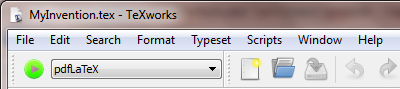
\includegraphics{TeXworks}
\par\end{centering}

\caption{\protect\TeX{}works ribbon bar}
\label{fig:TeXworks-ribbon-bar}
\end{figure}



\section{Driving \protect\LyX{}\label{sec:Driving-LyX}}

\LyX{}\index{LyX@\LyX{}} can be used to edit and produce your patent
application presuming you have:
\begin{itemize}
\item \LaTeX{} installed properly (remember \LyX{} is just a front-end for
\LaTeX{}).
\item \LyX{} installed properly.
\end{itemize}
Assuming you have followed the directions in \secref{Starting-a-New-Application},
you will have a directory called MyInvention\index{MyInvention file}
and in it you will have at least the files uspatent.cls, MyInvention.lyx,
Drawings.lyx, VisioDrawing.pdf, and TpXDrawing.tpx.

To edit your application, open MyInvention.lyx with \LyX{}.

If you created MyInvention.lyx by making a copy of PatentApplication.lyx,
then all of the document settings should be correctly configured (see
\ref{sub:LyX-Document-Settings} for a complete list of settings).

\begin{figure}
\begin{centering}

\includegraphics{LyX}
\par\end{centering}

\caption{\protect\LyX{} Output Controls}
\label{fig:LyX-output-controls}
\end{figure}
The output controls are shown in \figref{LyX-output-controls}. Pressing
the googly eyes to the left should cause \LyX{} to produce the PDF\index{PDF}
document and open it for display. For the display to work, you will
need to have a PDF reader installed.

You can learn more about \LyX{} on your own, but I have to call your
attention at this time to two key customizations that are unique to
the patent application layout:
\begin{itemize}
\item Environments\index{LyX@\LyX{}!environment}
\item Custom Insets\index{LyX@\LyX{}!custom inset}
\end{itemize}
The file uspatent.layout provided overrides and restricts the \emph{environments}
available in \LyX{}. To access these environments, click the drop-down
selector in the upper left corner of the \LyX{} editor dialog as shown
in \figref{LyX-environments}. Similarly, it provides \emph{custom
insets} that provide for certain cross-referencing features. To access
these, select them from the drop-down menu by selecting: \texttt{{[}Insert{]}{[}Custom
Insets{]}} as shown in \figref{LyX-custom-insets}.

\begin{figure}
\begin{centering}
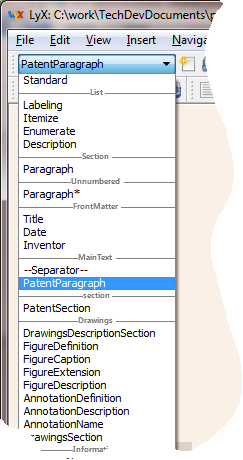
\includegraphics[scale=0.5]{LyXEnvironments}
\par\end{centering}

\caption{\protect\LyX{} Environments}
\index{environment}\index{LyX@\LyX{}!environment}\label{fig:LyX-environments}
\end{figure}
\begin{figure}
\begin{centering}
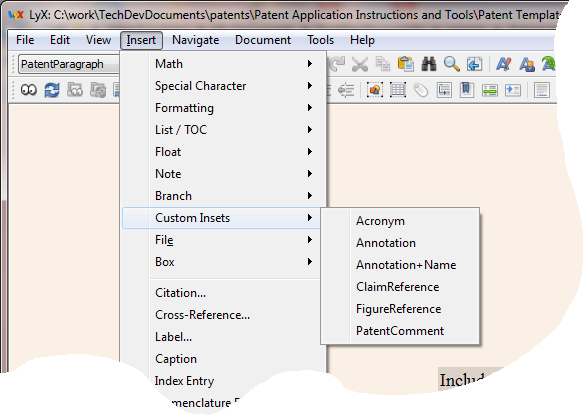
\includegraphics[scale=0.5]{LyXCustomInsets}
\par\end{centering}

\caption{\protect\LyX{} Custom Insets}
\label{fig:LyX-custom-insets}\index{LyX@\LyX{}!custom inset}\index{custom inset}
\end{figure}
The environments and custom insets are the full extent of the \LyX{}
customization and access all of the special patent application features.
These features are explained elsewhere in this document but I figured
you might want to know where to find them now.


\subsection{\protect\LyX{} Document Settings\label{sub:LyX-Document-Settings}}

\index{LyX@\LyX{}!document settings}If you start your new patent
application by renaming the PatentApplication.\LyX{} file and editing
it, you should never need to bother with any \LyX{} document settings
\emph{provided you don't change them}. \textbf{You are strongly encouraged
to not change \LyX{} document settings}. This section is provided
for completeness so that you know how \LyX{} is set up or in case
you get yourself in trouble.

Fortunately, for the most part, the default \LyX{} settings are used.
Also, since the application format is rigidly enforced from within
the \LaTeX{} class, most of the \LyX{} settings are overridden anyway.
This section contains the \LyX{} settings that are required.

\begin{figure}
\begin{centering}
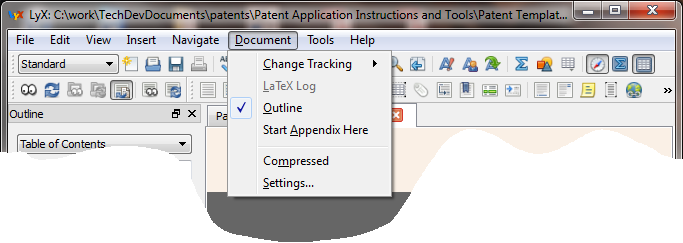
\includegraphics[scale=0.5]{DocumentSettings}
\par\end{centering}

\caption{\protect\LyX{} Document Settings}
\label{fig:LyX-document-settings}
\end{figure}
\LyX{} document settings are accessed via the Settings selection in
the Document drop-down menu using \texttt{{[}Document{]}{[}Settings{]}}
as shown in \figref{LyX-document-settings}.


\subsection{Document Class\label{sub:Document-Class}}

\begin{figure}
\begin{centering}
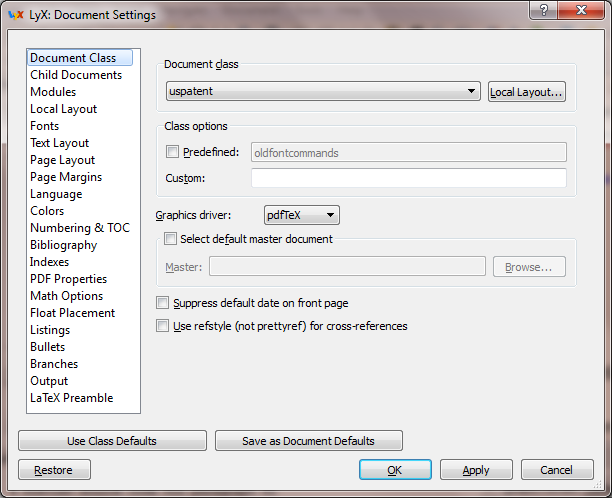
\includegraphics[scale=0.5]{LyXSettingsDocumentClass}
\par\end{centering}

\caption{\protect\LyX{} Document Class Settings}
\label{fig:LyX-document-class-settings}
\end{figure}
\index{LyX@\LyX{}!document class}Set the document class by pressing
the button labeled Local Layout and browsing to the uspatent.layout
file that must be located in the same directory as your patent application
file. Note that usually file classes and the associated layout files
are selected directly from the drop-down document class selection
button but our layout is local. You will be warned that things will
work properly only if the layout file is kept along with your patent
application file in the same directory. The Document Class dialog
is shown in \figref{LyX-document-class-settings}.


\subsection{Output Control - pdf\protect\LaTeX{}}

\begin{figure}
\begin{centering}
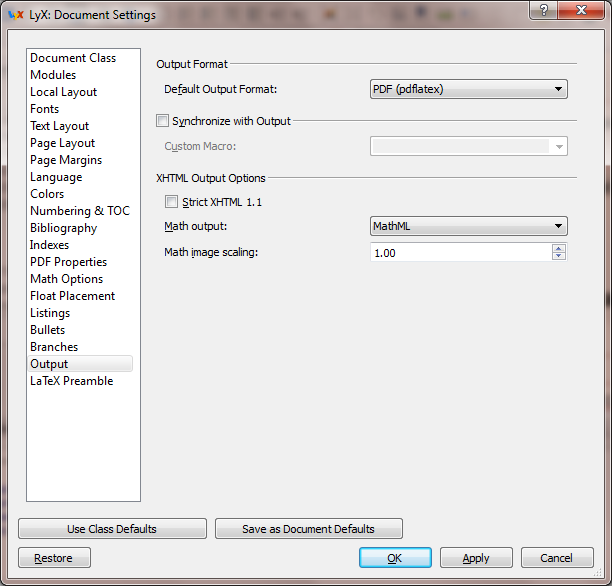
\includegraphics[scale=0.5]{LyXDocumentSettingsOutput}
\par\end{centering}

\caption{\protect\LyX{} Document Output Settings}
\label{fig:LyX-document-settings-output}\index{pdflatex}
\end{figure}
\begin{figure}
\begin{centering}
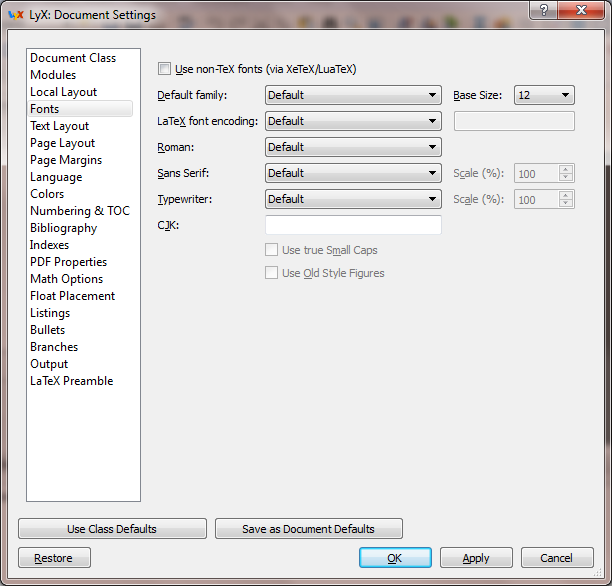
\includegraphics[scale=0.75]{LyXDocumentSettingsFont}
\par\end{centering}

\caption{\protect\LyX{} Document Font Settings}
\label{fig:LyX-document-settings-font}\index{pdflatex}
\end{figure}
\index{pdflatex}There are many offshoots from \LaTeX{} (see \subref{Installing-LaTeX});
we need to ensure that \LyX{} will choose pdf\LaTeX{} which is the
only output format that will work with the patent class file.

The output is selected from the Document Output Settings dialog as
shown in \figref{LyX-document-settings-output}. Under Output Format
select (PDF) pdflatex as the Default Output Format. There are other
settings that can prevent pdf\LaTeX{} as a choice. Make sure that
the ``use non-Tex fonts (via Xe\TeX{}/Lua\TeX{}) box'' is not checked
in the Document Fonts Settings menu as shown in \figref{LyX-document-settings-font}.


\section{The Layout of the Patent Application\label{sec:The-Layout-of-the-Patent-Application}}

Two possible \LaTeX{} patent application documents are shown in \figref{LaTeX-document-layout}
and \figref{LaTeX-document-layout-1}. Two possible corresponding
\LyX{} patent application documents are shown in \figref{LyX-document-layout}
and \figref{LyX-document-layout-1}.
\begin{figure}
\begin{centering}
\framebox{\begin{minipage}[t]{0.8\columnwidth}%
\texttt{\textbackslash{}documentclass{[}english{]}\{uspatent\} \%
includes the uspatent.cls class definitions}

\texttt{\medskip{}
}

\texttt{\ldots{}front matter\ldots{} \% all front matter definitions
go here\medskip{}
}

\texttt{\textbackslash{}include\{Drawings\} \% includes the figures
information}

\texttt{\medskip{}
}

\texttt{\textbackslash{}maketitle \% outputs the title and begins
the patent application}

\texttt{\medskip{}
}

\texttt{\textbackslash{}patentSection\{Field of the Invention\}}

\texttt{\textbackslash{}patentParagraph blah, blah blah \ldots{}}

\begin{center}
\texttt{\ldots{}}
\par\end{center}

\texttt{\textbackslash{}patentSection\{Cross Reference to Related
Applications\}}

\texttt{\textbackslash{}patentParagraph blah, blah blah \ldots{}}

\begin{center}
\texttt{\ldots{}}
\par\end{center}

\texttt{\textbackslash{}patentSection\{Background of the Invention\}}

\texttt{\textbackslash{}patentParagraph blah, blah blah \ldots{}}

\begin{center}
\texttt{\ldots{}}
\par\end{center}

\texttt{\textbackslash{}patentSection\{Objects of the Invention\}}

\texttt{\textbackslash{}patentParagraph blah, blah blah \ldots{}}

\begin{center}
\texttt{\ldots{}}
\par\end{center}

\texttt{\textbackslash{}patentSection\{Summary of the Invention\}}

\texttt{\textbackslash{}patentParagraph blah, blah blah \ldots{}}

\begin{center}
\texttt{\ldots{}}
\par\end{center}

\texttt{\textbackslash{}patentDrawingDescriptions}

\texttt{\medskip{}
}

\texttt{\textbackslash{}patentSection\{Detailed Description of the
Preferred Embodiments\}}

\texttt{\textbackslash{}patentParagraph blah, blah blah \ldots{}}

\begin{center}
\texttt{\ldots{}}
\par\end{center}

\texttt{\textbackslash{}patentClaimsStart}

\texttt{\ldots{}}

\texttt{\textbackslash{}patentClaimsEnd}

\texttt{\medskip{}
}

\texttt{\textbackslash{}patentSection\{Abstract\}}

\texttt{\textbackslash{}patentParagraph blah, blah blah \ldots{}}

\begin{center}
\texttt{\ldots{}}
\par\end{center}

\texttt{\textbackslash{}patentDrawings}

\texttt{\medskip{}
}

\texttt{\textbackslash{}end\{document\}}%
\end{minipage}}
\par\end{centering}

\caption{Skeleton \protect\LaTeX{} Patent Application Document}
\label{fig:LaTeX-document-layout}\index{LaTeX@\LaTeX{}!layout}\index{maketitle macro@\textbackslash{}maketitle macro}\index{LaTeX@\LaTeX{}!macro!maketitle@\textbackslash{}maketitle}\index{patentDrawings macro@\textbackslash{}patentDrawings macro}\index{LaTeX@\LaTeX{}!macro!patentDrawings@\textbackslash{}patentDrawings}\index{patentDrawingDescriptions macro@\textbackslash{}patentDrawingDescriptions macro}\index{LaTeX@\LaTeX{}!macro!patentDrawingDescriptions@\textbackslash{}patentDrawingDescriptions}\index{patentParagraph macro@\textbackslash{}patentParagraph macro}\index{LaTeX@\LaTeX{}!macro!patentParagraph@\textbackslash{}patentParagraph}\index{patentSection macro@\textbackslash{}patentSection macro}\index{LaTeX@\LaTeX{}!macro!patentSection@\textbackslash{}patentSection}\index{patentClaimsStart macro@\textbackslash{}patentClaimsStart macro}\index{LaTeX@\LaTeX{}!macro!patentClaimsStart@\textbackslash{}patentClaimsStart}\index{patentClaimsEnd macro@\textbackslash{}patentClaimsEnd macro}\index{LaTeX@\LaTeX{}!macro!patentClaimsEnd@\textbackslash{}patentClaimsEnd}\index{end{document} macro@\textbackslash{}end\{document\} macro}\index{LaTeX@\LaTeX{}!macro!end{document}@\textbackslash{}end\{document\}}\index{front matter}\index{uspatent.cls}\index{documentclass macro@\textbackslash{}documentclass macro}\index{LaTeX@\LaTeX{}!macro!documentclass@\textbackslash{}documentclass}
\end{figure}
\begin{figure}
\begin{centering}
\framebox{\begin{minipage}[t]{0.8\columnwidth}%
\texttt{\textbackslash{}documentclass{[}english{]}\{uspatent\} \%
includes the uspatent.cls class definitions}

\texttt{\medskip{}
}

\texttt{\ldots{}front matter\ldots{} \% all front matter definitions
go here\medskip{}
}

\texttt{\textbackslash{}include\{Drawings\} \% includes the figures
information}

\texttt{\medskip{}
}

\texttt{\textbackslash{}maketitle \% outputs the title and begins
the patent application}

\texttt{\medskip{}
}

\texttt{\textbackslash{}patentSection\{Technical Field\}}

\texttt{\textbackslash{}patentParagraph blah, blah blah \ldots{}}

\begin{center}
\texttt{\ldots{}}
\par\end{center}

\texttt{\textbackslash{}patentSection\{Cross Reference to Related
Applications\}}

\texttt{\textbackslash{}patentParagraph blah, blah blah \ldots{}}

\begin{center}
\texttt{\ldots{}}
\par\end{center}

\texttt{\textbackslash{}patentSection\{Background\}}

\texttt{\textbackslash{}patentParagraph blah, blah blah \ldots{}}

\begin{center}
\texttt{\ldots{}}
\par\end{center}

\texttt{\textbackslash{}patentSection\{Summary\}}

\texttt{\textbackslash{}patentParagraph blah, blah blah \ldots{}}

\begin{center}
\texttt{\ldots{}}
\par\end{center}

\texttt{\textbackslash{}patentDrawingDescriptions}

\texttt{\medskip{}
}

\texttt{\textbackslash{}patentSection\{Detailed Description\}}

\texttt{\textbackslash{}patentParagraph blah, blah blah \ldots{}}

\begin{center}
\texttt{\ldots{}}
\par\end{center}

\texttt{\textbackslash{}patentClaimsStart}

\texttt{\ldots{}}

\texttt{\textbackslash{}patentClaimsEnd}

\texttt{\medskip{}
}

\texttt{\textbackslash{}patentSection\{Abstract\}}

\texttt{\textbackslash{}patentParagraph blah, blah blah \ldots{}}

\begin{center}
\texttt{\ldots{}}
\par\end{center}

\texttt{\textbackslash{}patentDrawings}

\texttt{\medskip{}
}

\texttt{\textbackslash{}end\{document\}}%
\end{minipage}}
\par\end{centering}

\caption{Skeleton \protect\LaTeX{} Patent Application Document}
\label{fig:LaTeX-document-layout-1}\index{LaTeX@\LaTeX{}!layout}\index{maketitle macro@\textbackslash{}maketitle macro}\index{LaTeX@\LaTeX{}!macro!maketitle@\textbackslash{}maketitle}\index{patentDrawings macro@\textbackslash{}patentDrawings macro}\index{LaTeX@\LaTeX{}!macro!patentDrawings@\textbackslash{}patentDrawings}\index{patentDrawingDescriptions macro@\textbackslash{}patentDrawingDescriptions macro}\index{LaTeX@\LaTeX{}!macro!patentDrawingDescriptions@\textbackslash{}patentDrawingDescriptions}\index{patentParagraph macro@\textbackslash{}patentParagraph macro}\index{LaTeX@\LaTeX{}!macro!patentParagraph@\textbackslash{}patentParagraph}\index{patentSection macro@\textbackslash{}patentSection macro}\index{LaTeX@\LaTeX{}!macro!patentSection@\textbackslash{}patentSection}\index{patentClaimsStart macro@\textbackslash{}patentClaimsStart macro}\index{LaTeX@\LaTeX{}!macro!patentClaimsStart@\textbackslash{}patentClaimsStart}\index{patentClaimsEnd macro@\textbackslash{}patentClaimsEnd macro}\index{LaTeX@\LaTeX{}!macro!patentClaimsEnd@\textbackslash{}patentClaimsEnd}\index{end{document} macro@\textbackslash{}end\{document\} macro}\index{LaTeX@\LaTeX{}!macro!end{document}@\textbackslash{}end\{document\}}\index{front matter}\index{uspatent.cls}\index{documentclass macro@\textbackslash{}documentclass macro}\index{LaTeX@\LaTeX{}!macro!documentclass@\textbackslash{}documentclass}
\end{figure}
\begin{figure}
\begin{centering}
\framebox{\begin{minipage}[t]{0.8\columnwidth}%
\begin{flushright}
\ldots{}front matter\ldots{} \medskip{}

\par\end{flushright}

\begin{center}
\framebox{\begin{minipage}[t]{0.3\columnwidth}%
\begin{center}
Include: Drawings.lyx
\par\end{center}%
\end{minipage}}
\par\end{center}

\medskip{}


\begin{center}
\textbf{\textsc{\uline{Field of the Invention}}}
\par\end{center}

blah, blah blah \ldots{}\medskip{}


\begin{center}
\textbf{\textsc{\uline{Cross Reference to Related Applications}}}
\par\end{center}

blah, blah blah \ldots{}

\medskip{}


\begin{center}
\textbf{\textsc{\uline{Background of the Invention}}}
\par\end{center}

blah, blah blah \ldots{}

\medskip{}


\begin{center}
\textbf{\textsc{\uline{Objects of the Invention}}}
\par\end{center}

blah, blah blah \ldots{}

\medskip{}


\begin{center}
\textbf{\textsc{\uline{Summary of the Invention}}}
\par\end{center}

blah, blah blah \ldots{}

\medskip{}


\begin{flushright}
\textbf{\tiny ---BRIEF DESCRIPTION OF THE DRAWINGS---}
\par\end{flushright}{\tiny \par}

\medskip{}


\begin{center}
\textbf{\textsc{\uline{Detailed Description of the Preferred Embodiments}}}
\par\end{center}

blah, blah blah \ldots{}

\medskip{}


\begin{flushright}
\textbf{\tiny ---START OF PATENT CLAIMS---}
\par\end{flushright}{\tiny \par}

\begin{center}
\ldots{}
\par\end{center}

\begin{flushright}
\textbf{\tiny ---END OF PATENT CLAIMS---}
\par\end{flushright}{\tiny \par}

\medskip{}


\begin{center}
\textbf{\textsc{\uline{Abstract}}}
\par\end{center}

blah, blah blah \ldots{}

\medskip{}


\begin{flushright}
\textbf{\tiny ---PATENT DRAWINGS---}
\par\end{flushright}%
\end{minipage}}
\par\end{centering}

\caption{Skeleton \protect\LyX{} Patent Application Document}
\label{fig:LyX-document-layout}\index{LyX@\LyX{}!layout}\index{front matter}\index{PatentSection environment}\index{LyX@\LyX{}!environment!PatentSection}\index{PatentParagraph environment}\index{LyX@\LyX{}!environment!PatentParagraph}\index{DrawingsDescriptionSection environment}\index{LyX@\LyX{}!environment!DrawingsDescriptionSection}\index{DrawingsSection environment}\index{LyX@\LyX{}!environment!DrawingsSection}\index{ClaimsStart environment}\index{LyX@\LyX{}!environment!ClaimsStart}\index{ClaimsEnd environment}\index{LyX@\LyX{}!environment!ClaimsEnd}
\end{figure}
\begin{figure}
\begin{centering}
\framebox{\begin{minipage}[t]{0.8\columnwidth}%
\begin{flushright}
\ldots{}front matter\ldots{} \medskip{}

\par\end{flushright}

\begin{center}
\framebox{\begin{minipage}[t]{0.3\columnwidth}%
\begin{center}
Include: Drawings.lyx
\par\end{center}%
\end{minipage}}
\par\end{center}

\medskip{}


\begin{center}
\textbf{\textsc{\uline{Technical Field}}}
\par\end{center}

blah, blah blah \ldots{}\medskip{}


\begin{center}
\textbf{\textsc{\uline{Cross Reference to Related Applications}}}
\par\end{center}

blah, blah blah \ldots{}

\medskip{}


\begin{center}
\textbf{\textsc{\uline{Background}}}
\par\end{center}

blah, blah blah \ldots{}

\medskip{}


\begin{center}
\textbf{\textsc{\uline{Summary}}}
\par\end{center}

blah, blah blah \ldots{}

\medskip{}


\begin{flushright}
\textbf{\tiny ---BRIEF DESCRIPTION OF THE DRAWINGS---}
\par\end{flushright}{\tiny \par}

\medskip{}


\begin{center}
\textbf{\textsc{\uline{Detailed Description}}}
\par\end{center}

blah, blah blah \ldots{}

\medskip{}


\begin{flushright}
\textbf{\tiny ---START OF PATENT CLAIMS---}
\par\end{flushright}{\tiny \par}

\begin{center}
\ldots{}
\par\end{center}

\begin{flushright}
\textbf{\tiny ---END OF PATENT CLAIMS---}
\par\end{flushright}{\tiny \par}

\medskip{}


\begin{center}
\textbf{\textsc{\uline{Abstract}}}
\par\end{center}

blah, blah blah \ldots{}

\medskip{}


\begin{flushright}
\textbf{\tiny ---PATENT DRAWINGS---}
\par\end{flushright}%
\end{minipage}}
\par\end{centering}

\caption{Skeleton \protect\LyX{} Patent Application Document}
\label{fig:LyX-document-layout-1}\index{LyX@\LyX{}!layout}\index{front matter}\index{PatentSection environment}\index{LyX@\LyX{}!environment!PatentSection}\index{PatentParagraph environment}\index{LyX@\LyX{}!environment!PatentParagraph}\index{DrawingsDescriptionSection environment}\index{LyX@\LyX{}!environment!DrawingsDescriptionSection}\index{DrawingsSection environment}\index{LyX@\LyX{}!environment!DrawingsSection}\index{ClaimsStart environment}\index{LyX@\LyX{}!environment!ClaimsStart}\index{ClaimsEnd environment}\index{LyX@\LyX{}!environment!ClaimsEnd}
\end{figure}
 There are two styles to reflect the tastes of patent lawyers who
reviewed this document. I use the first layout style.

\index{LaTeX@\LaTeX{}!layout}The \LaTeX{} document starts with a
declaration of the uspatent class. Every \LaTeX{} document must contain
at least one of these declarations and here we specify the file containing
the typesetting and macro definitions that are used in the patent
application. It ends with an \texttt{\textbackslash{}end\{document\}}
\index{end{document} macro@\textbackslash{}end\{document\} macro}\index{LaTeX@\LaTeX{}!macro!end{document}@\textbackslash{}end\{document\}}statement.
After the class definition, there are various \index{front matter}front
matter definitions (see \secref{Front-matter}) that define things
like the title, inventor, etc. This is followed by an inclusion of
a drawings file. This file defines how the drawings will be read in,
described, annotated, etc. See \secref{Drawings} for information
on how drawings are controlled. After the drawings, we see the \texttt{\textbackslash{}maketitle}
\index{maketitle macro@\textbackslash{}maketitle macro}\index{LaTeX@\LaTeX{}!macro!maketitle@\textbackslash{}maketitle}macro
which is described in \secref{Front-matter}. This macro defines where
the title page should be printed and where the patent sections start.
The remainder of the patent application consists mostly of patent
sections set off by the\index{patentSection macro@\textbackslash{}patentSection macro}\index{LaTeX@\LaTeX{}!macro!patentSection@\textbackslash{}patentSection}
\texttt{\textbackslash{}patentSection} macro described in \subref{Patent-Sections}.
Each section consists of one or more paragraphs where each paragraph
begins with \texttt{\textbackslash{}patentParagraph} \index{patentParagraph macro@\textbackslash{}patentParagraph macro}\index{LaTeX@\LaTeX{}!macro!patentParagraph@\textbackslash{}patentParagraph}(see
\subref{Paragraph-Numbering}). You will notice two macros that control
drawings:\index{patentDrawings macro@\textbackslash{}patentDrawings macro}\index{LaTeX@\LaTeX{}!macro!patentDrawings@\textbackslash{}patentDrawings}\index{patentDrawingDescriptions macro@\textbackslash{}patentDrawingDescriptions macro}\index{LaTeX@\LaTeX{}!macro!patentDrawingDescriptions@\textbackslash{}patentDrawingDescriptions}
\texttt{\textbackslash{}patentDrawingDescriptions} and \texttt{\textbackslash{}patentDrawings}.
These macros expand into automatically generated sections containing
a brief description of the drawings and the drawings themselves. The
control of drawings is explained in \secref{Drawings}. Finally, you
will notice two macros that delimit the area where the patent claims
are placed:\index{patentClaimsStart macro@\textbackslash{}patentClaimsStart macro}\index{LaTeX@\LaTeX{}!macro!patentClaimsStart@\textbackslash{}patentClaimsStart}\index{patentClaimsEnd macro@\textbackslash{}patentClaimsEnd macro}\index{LaTeX@\LaTeX{}!macro!patentClaimsEnd@\textbackslash{}patentClaimsEnd}
\texttt{\textbackslash{}patentClaimsStart} and \texttt{\textbackslash{}patentClaimsEnd}.
The formatting of claims is described in \secref{Claims}.

\index{LyX@\LyX{}!layout}The \LyX{} document starts directly with
the various front matter\index{front matter} definitions (see \secref{Front-matter})
that define things like the title, inventor, etc. This is followed
by an inclusion of a drawings file. This file defines how the drawings
will be read in, described, annotated, etc. See \secref{Drawings}
for information on how drawings are controlled. The remainder of the
patent application consists mostly of patent sections formatted by
the \textbf{PatentSection} environment\index{PatentSection environment}\index{LyX@\LyX{}!environment!PatentSection}
described in \subref{Patent-Sections}. Each section consists of one
or more paragraphs where each paragraph is formatted with the\index{PatentParagraph environment}\index{LyX@\LyX{}!environment!PatentParagraph}
\textbf{PatentParagraph} environment (see \subref{Paragraph-Numbering}).
You will notice two environments that control drawings: \textbf{\footnotesize ---BRIEF
DESCRIPTION OF THE DRAWINGS--} and \textbf{\footnotesize ---PATENT
DRAWINGS---}. \index{DrawingsDescriptionSection environment}\index{LyX@\LyX{}!environment!DrawingsDescriptionSection}\index{DrawingsSection environment}\index{LyX@\LyX{}!environment!DrawingsSection}These
environments expand into automatically generated sections containing
a brief description of the drawings and the drawings themselves. The
control of drawings is explained in \secref{Drawings}. Finally, you
will notice two environments that delimit the area where the patent
claims are placed:\index{ClaimsStart environment}\index{LyX@\LyX{}!environment!ClaimsStart}\index{ClaimsEnd environment}\index{LyX@\LyX{}!environment!ClaimsEnd}
\textbf{\footnotesize ---START OF PATENT CLAIMS---} and \textbf{\footnotesize ---END
OF PATENT CLAIMS---}. The formatting of claims is described in \secref{Claims}.


\section{Front Matter\label{sec:Front-matter}}

\index{front matter}Front matter is, as the name indicates, information
that must appear at or near the front of the document. The information
must be provided prior to the title (see \subref{Title}), date (see
\subref{Date}), and inventor name (see \subref{Inventor-Name(s)})
in \LyX{} documents, because \LyX{} will expect to emit the title
page immediately following the last of these three definitions. In
\LaTeX{}, the emission of the title page is determined by the location
of the \texttt{\textbackslash{}maketitle}{\Large{} }macro.

Thus in \LyX{}, the front matter appears like:\index{Title environment}\index{LyX@\LyX{}!environment!Title}\index{Date environment}\index{LyX@\LyX{}!environment!Date}\index{Inventor environment}\index{LyX@\LyX{}!environment!Inventor}

\begin{center}
\framebox{\begin{minipage}[t]{0.6\columnwidth}%
\begin{flushright}
\textbf{\small \ldots{}}\linebreak{}
\textbf{\small various front matter definitions}\linebreak{}
\textbf{\small \ldots{}}
\par\end{flushright}{\small \par}

\begin{center}
\textbf{\Large Invention Name Here}
\par\end{center}{\Large \par}

\begin{center}
June 3, 2012
\par\end{center}

\begin{center}
Peter J. Pupalaikis
\par\end{center}%
\end{minipage}}
\par\end{center}

As mentioned, in \LyX{}, the end of the front matter and title page
information is delimited by the last of the invention name, date,
and inventor.

In \LaTeX{}, the front matter appears like:\index{maketitle macro@\textbackslash{}maketitle macro}\index{LaTeX@\LaTeX{}!macro!maketitle@\textbackslash{}maketitle}\index{documentclass macro@\textbackslash{}documentclass macro}\index{LaTeX@\LaTeX{}!macro!documentclass@\textbackslash{}documentclass}\index{title macro@\textbackslash{}title macro}\index{LaTeX@\LaTeX{}!macro!title@\textbackslash{}title}\index{date macro@\textbackslash{}date macro}\index{LaTeX@\LaTeX{}!macro!date@\textbackslash{}date}\index{inventor macro@\textbackslash{}inventor macro}\index{LaTeX@\LaTeX{}!macro!inventor@\textbackslash{}inventor}

\begin{center}
\framebox{\begin{minipage}[t]{0.6\columnwidth}%
\texttt{\textbackslash{}documentclass{[}english{]}\{uspatent\}}

\begin{flushleft}
\texttt{\ldots{}}~\\
\texttt{various front matter definitions}~\\
\texttt{\ldots{}}
\par\end{flushleft}

\begin{flushleft}
\texttt{\textbackslash{}title\{Invention Name Here\}}~\\
\texttt{\textbackslash{}date\{June 3, 2012\}}~\\
\texttt{\textbackslash{}inventor\{Peter J. Pupalaikis\}}
\par\end{flushleft}

\texttt{\textbackslash{}maketitle}%
\end{minipage}}
\par\end{center}

Here we see that the \texttt{\textbackslash{}maketitle} macro defines
the end of the front matter and title page definitions.

In case you are wondering, your patent application will look nothing
like it looks in the \LyX{} editor with the title followed by the
date followed by the inventor name. This is what is meant by WYSIWYM.
You know that you need all of this information and it needs to go
somewhere. \LyX{} provides the method of entering this information
and later when you compile the document, you'll see where it actually
goes.


\subsection{Assignee Information}

The assignee\index{assignee} is the name of the entity that will
own the rights to the invention. Typically this is the company for
which the inventor works. The assignee information is defined using:
\begin{itemize}
\item \begin{sloppypar}The \index{assignee name}assignee name is defined
using the \texttt{\textbackslash{}setAssigneeName} \index{setAssigneeName macro@\textbackslash{}setAssigneeName macro}\index{LaTeX@\LaTeX{}!macro!setAssigneeName@\textbackslash{}setAssigneeName}macro
in \LaTeX{} or the \textbf{AssigneeName} \index{AssigneeName environment}\index{LyX@\LyX{}!environment!AssigneeName}environment
in \LyX{}.\end{sloppypar}
\item \begin{sloppypar}The assignee address\index{assignee address} is
defined using the \texttt{\textbackslash{}setAssigneeAddress} \index{setAssigneeAddress macro@\textbackslash{}setAssigneeAddress macro}\index{LaTeX@\LaTeX{}!macro!setAssigneeAddress@\textbackslash{}setAssigneeAddress}macro
in \LaTeX{} or the \textbf{AssigneeAddress} \index{AssigneeAddress environment}\index{LyX@\LyX{}!environment!AssigneeAddress}environment
in \LyX{}.\end{sloppypar}
\item \begin{sloppypar}The assignee city\index{assignee city}, state \&
zip code is defined using the \textbackslash{}setAssigneeCity \index{setAssigneeCity macro@\textbackslash{}setAssigneeCity macro}\index{LaTeX@\LaTeX{}!macro!setAssigneeCity@\textbackslash{}setAssigneeCity}macro
in \LaTeX{} or the \textbf{AssigneeCity} \index{AssigneeCity environment}\index{LyX@\LyX{}!environment!AssigneeCity}environment
in \LyX{}.\end{sloppypar}
\item \begin{sloppypar}The assignee phone number\index{assignee phone number}
is defined using the \texttt{\textbackslash{}setAssigneePhone} \index{setAssigneePhone macro@\textbackslash{}setAssigneePhone macro}\index{LaTeX@\LaTeX{}!macro!setAssigneePhone@\textbackslash{}setAssigneePhone}macro
in \LaTeX{} or the \textbf{AssigneePhone} \index{AssigneePhone environment}\index{LyX@\LyX{}!environment!AssigneePhone}environment
in \LyX{}.\end{sloppypar}
\end{itemize}
Here is an example \LyX{} assignee definition:

\begin{center}
\framebox{\begin{minipage}[t]{0.6\columnwidth}%
\begin{flushright}
\textbf{\small Assignee Name:Company Name}\linebreak{}
\textbf{\small Assignee Address:Number and Street Name}\linebreak{}
\textbf{\small Assignee City:City, State and Zip}\linebreak{}
\textbf{\small Assignee Phone:Telephone Number}
\par\end{flushright}%
\end{minipage}}
\par\end{center}

\noindent \index{AssigneeName environment}\index{LyX@\LyX{}!environment!AssigneeName}\index{AssigneeAddress environment}\index{LyX@\LyX{}!environment!AssigneeAddress}\index{AssigneeCity environment}\index{LyX@\LyX{}!environment!AssigneeCity}\index{AssigneePhone environment}\index{LyX@\LyX{}!environment!AssigneePhone}

Here is an example \LaTeX{} assignee definition:

\begin{center}
\framebox{\begin{minipage}[t]{0.6\columnwidth}%
\begin{flushleft}
\texttt{\textbackslash{}setAssigneeName\{Company Name\}}~\\
\texttt{\textbackslash{}setAssigneeAddress\{Number and Street Name\}}~\\
\texttt{\textbackslash{}setAssigneeCity\{City, State and Zip\}}~\\
\texttt{\textbackslash{}setAssigneePhone\{Telephone Number\}}
\par\end{flushleft}%
\end{minipage}}
\par\end{center}

\noindent \index{setAssigneeName macro@\textbackslash{}setAssigneeName macro}\index{LaTeX@\LaTeX{}!macro!setAssigneeName@\textbackslash{}setAssigneeName}\index{setAssigneeAddress macro@\textbackslash{}setAssigneeAddress macro}\index{LaTeX@\LaTeX{}!macro!setAssigneeAddress@\textbackslash{}setAssigneeAddress}\index{setAssigneeCity macro@\textbackslash{}setAssigneeCity macro}\index{LaTeX@\LaTeX{}!macro!setAssigneeCity@\textbackslash{}setAssigneeCity}\index{setAssigneePhone macro@\textbackslash{}setAssigneePhone macro}\index{LaTeX@\LaTeX{}!macro!setAssigneePhone@\textbackslash{}setAssigneePhone}I
have been advised that some patent attorneys prefer not to include
the assignee information in the patent application. If you or your
patent attorney prefers not to provide this information, then simply
don't define these fields. You should note, however, that in draft
mode (see \ref{sub:Printing-Mode}), the patent prints with a confidential
heading which does not print if the assignee name has not been defined.


\subsection{Patent Lawyer Information}

\index{patent lawyer}The patent lawyer information is defined using:
\begin{itemize}
\item \begin{sloppypar}The lawyer name is defined using the \texttt{\textbackslash{}setLawyerName}
\index{setLawyerName macro@\textbackslash{}setLawyerName macro}\index{LaTeX@\LaTeX{}!macro!setLawyerName@\textbackslash{}setLawyerName}macro
in \LaTeX{} or the \textbf{LawyerName} \index{LawyerName environment}\index{LyX@\LyX{}!environment!LawyerName}environment
in \LyX{}.\end{sloppypar}
\item \begin{sloppypar}The lawyer registration number is defined using
the \texttt{\textbackslash{}setLawyerNumber} \index{setLawyerNumber macro@\textbackslash{}setLawyerNumber macro}\index{LaTeX@\LaTeX{}!macro!setLawyerNumber@\textbackslash{}setLawyerNumber}macro
in \LaTeX{} or the \textbf{LawyerNumber} \index{LawyerNumber environment}\index{LyX@\LyX{}!environment!LawyerNumber}environment
in \LyX{}.\end{sloppypar}
\item \begin{sloppypar}The lawyer phone number is defined using the \texttt{\textbackslash{}setLawyerPhone}
\index{setLawyerPhone macro@\textbackslash{}setLawyerPhone macro}\index{LaTeX@\LaTeX{}!macro!setLawyerPhone@\textbackslash{}setLawyerPhone}macro
in \LaTeX{} or the \textbf{LawyerPhone} \index{LawyerPhone environment}\index{LyX@\LyX{}!environment!LawyerPhone}environment
in \LyX{}.\end{sloppypar}
\end{itemize}
Here is an example \LyX{} patent lawyer definition:

\begin{center}
\textbf{\small }%
\framebox{\begin{minipage}[t]{0.6\columnwidth}%
\begin{flushright}
\textbf{\small Patent Lawyer Name:First M. Last}\linebreak{}
\textbf{\small Patent Lawyer Reg Number: \#:99,999}\linebreak{}
\textbf{\small Patent Lawyer Phone:(845) 555-2000}
\par\end{flushright}%
\end{minipage}}
\par\end{center}{\small \par}

\noindent \index{LawyerName environment}\index{LyX@\LyX{}!environment!LawyerName}\index{LawyerNumber environment}\index{LyX@\LyX{}!environment!LawyerNumber}\index{LawyerPhone environment}\index{LyX@\LyX{}!environment!LawyerPhone}

Here is an example \LaTeX{} assignee definition:

\begin{center}
\framebox{\begin{minipage}[t]{0.6\columnwidth}%
\begin{flushleft}
\textbackslash{}setLawyerName\{First M. Last\}\texttt{}~\\
\textbackslash{}setLawyerNumber\{Reg \textbackslash{}\#:99,999\}\texttt{}~\\
\textbackslash{}setLawyerPhone\{845-555-2000\}
\par\end{flushleft}%
\end{minipage}}
\par\end{center}

\noindent \index{setLawyerName macro@\textbackslash{}setLawyerName macro}\index{LaTeX@\LaTeX{}!macro!setLawyerName@\textbackslash{}setLawyerName}\index{setLawyerNumber macro@\textbackslash{}setLawyerNumber macro}\index{LaTeX@\LaTeX{}!macro!setLawyerNumber@\textbackslash{}setLawyerNumber}\index{setLawyerPhone macro@\textbackslash{}setLawyerPhone macro}\index{LaTeX@\LaTeX{}!macro!setLawyerPhone@\textbackslash{}setLawyerPhone}I
have been advised that some patent attorneys prefer not to include
the patent lawyer information in the patent application. If you or
your patent attorney prefers not to provide this information, then
simply don't define these fields.


\subsection{Docket Number}

\index{docket number}To track the progress of a patent during prosecution,
a patent application is assigned a \emph{docket number}. This is the
number that you refer to internal to your company. At my company,
this number is provided by the paralegal handling patent applications.
When we are planning on filing an application, she provides a new
number to use.

We use a numbering scheme which is in the form LEC-YY-1NN0-U1 where
YY is the last two digits of the year, NN is the number of the patent
filed this year, and U or D is used depending on whether the invention
is a design or utility patent. By the way, the classes, layouts and
all of this documentation pertains only to utility patent applications.
Sometimes the number after the U is used to distinguish related applications
such as continuations, provisionals and divisionals. You will need
to find out this numbering scheme at your company and how these numbers
are assigned.

The application number is defined using the \texttt{\textbackslash{}setDocketNumber}
\index{setDocketNumber macro@\textbackslash{}setDocketNumber macro}\index{LaTeX@\LaTeX{}!macro!setDocketNumber@\textbackslash{}setDocketNumber}macro
in \LaTeX{} or the \textbf{DocketNumber} \index{DocketNumber environment}\index{LyX@\LyX{}!environment!DocketNumber}environment
in \LyX{}.

Here is an example \LyX{} document docket number definition:

\begin{center}
\framebox{\begin{minipage}[t]{0.6\columnwidth}%
\begin{flushright}
\textbf{\small Docket Number:LEC-YY-1NN0-U1}
\par\end{flushright}%
\end{minipage}}
\par\end{center}

\index{DocketNumber environment}\index{LyX@\LyX{}!environment!DocketNumber}

Here is an example \LaTeX{} document docket number definition:

\begin{center}
\framebox{\begin{minipage}[t]{0.6\columnwidth}%
\begin{flushleft}
\texttt{\textbackslash{}setDocketNumber\{LEC-YY-1NN0-U1\}}
\par\end{flushleft}%
\end{minipage}}
\par\end{center}

\index{setDocketNumber macro@\textbackslash{}setDocketNumber macro}\index{LaTeX@\LaTeX{}!macro!setDocketNumber@\textbackslash{}setDocketNumber}If
you do not have and never will have a docket number, simply don't
define it.


\subsection{DocumentVersion}

The document version is defined using the \texttt{\textbackslash{}setDocumentVersion}
\index{setDocumentVersion macro@\textbackslash{}setDocumentVersion macro}\index{LaTeX@\LaTeX{}!macro!setDocumentVersion@\textbackslash{}setDocumentVersion}macro
in \LaTeX{} or the \textbf{DocumentVersion} \index{DocumentVersion environment}\index{LyX@\LyX{}!environment!DocumentVersion}environment
in \LyX{}. The argument is x.y where x is the major version number
and y is the minor version number. This version number is only printed
in draft mode.

Here is an example \LyX{} document version definition:

\begin{center}
\framebox{\begin{minipage}[t]{0.6\columnwidth}%
\begin{flushright}
\textbf{\small Version:0.0}
\par\end{flushright}%
\end{minipage}}
\par\end{center}

\index{DocumentVersion environment}\index{LyX@\LyX{}!environment!DocumentVersion}

Here is an example \LaTeX{} document version definition:

\begin{center}
\framebox{\begin{minipage}[t]{0.6\columnwidth}%
\begin{flushleft}
\texttt{\textbackslash{}setDocumentVersion\{0.0\}}
\par\end{flushleft}%
\end{minipage}}
\par\end{center}

\index{setDocumentVersion macro@\textbackslash{}setDocumentVersion macro}\index{LaTeX@\LaTeX{}!macro!setDocumentVersion@\textbackslash{}setDocumentVersion}If
you do not supply a version number, a value of 0.0 is supplied for
you.


\subsection{Inventor Name(s)\label{sub:Inventor-Name(s)}}

\index{inventor name}Inventions often include multiple inventors.
All inventors are considered equal from the view of the patent office
regardless of the order in which they are listed. That being said,
the first inventor named gets some additional prestige factor in that
the patent is referred to in many places as invented by the first
named inventor suffixed with ``et al.''. The drawing section also
contains only the first named inventor (see \subref{The-Drawings-Section}).

The first named inventor is assigned differently from all of the other
inventors and is assigned using the \texttt{\textbackslash{}inventor}
\index{inventor macro@\textbackslash{}inventor macro}\index{LaTeX@\LaTeX{}!macro!inventor@\textbackslash{}inventor}macro
in \LaTeX{} or the \textbf{Inventor} \index{Inventor environment}\index{LyX@\LyX{}!environment!Inventor}environment
in \LyX{}. In \LaTeX{} and \LyX{}, the first named inventor is generally
assigned under the invention title and date. Other inventors are assigned
using the \texttt{\textbackslash{}setOtherInventor} \index{setOtherInventor macro@\textbackslash{}setOtherInventor macro}\index{LaTeX@\LaTeX{}!macro!setOtherInventor@\textbackslash{}setOtherInventor}macro
in \LaTeX{} or the \textbf{OtherInventor} \index{OtherInventor environment}\index{LyX@\LyX{}!environment!OtherInventor}environment
in \LyX{}. These assignments are made in the front matter prior to
the invention title, date and first inventor. \LaTeX{} keeps track
of all of the inventors added, so the same macro is used to assign
each one. The title page output during compilation provides a list
starting with the first inventor followed by the other inventors in
the order that they are listed. The uspatent.cls \LaTeX{} class file
provides for up to eight inventors before the title page production
fails.

Here is an example \LyX{} inventors definition:

\begin{center}
\framebox{\begin{minipage}[t]{0.6\columnwidth}%
\begin{flushright}
\textbf{\small OtherInventor:John D. Smith}\linebreak{}
\textbf{\small OtherInventor:Sally G. Jones}\linebreak{}
\textbf{\small OtherInventor:Samuel J. Jackson}
\par\end{flushright}{\small \par}

\begin{center}
\textbf{\Large Invention Name Here}
\par\end{center}{\Large \par}

\begin{center}
June 3, 2012
\par\end{center}

\begin{center}
Peter J. Pupalaikis
\par\end{center}%
\end{minipage}}
\par\end{center}

\index{OtherInventor environment}\index{LyX@\LyX{}!environment!OtherInventor}\index{Inventor environment}\index{LyX@\LyX{}!environment!Inventor}

Here is an example \LaTeX{} inventors definition:

\begin{center}
\framebox{\begin{minipage}[t]{0.6\columnwidth}%
\begin{flushleft}
\texttt{\textbackslash{}setOtherInventor\{John D. Smith\}}~\\
\texttt{\textbackslash{}setOtherInventor\{Sally G. Jones\}}~\\
\texttt{\textbackslash{}setOtherInventor\{Samuel J. Jackson\}}
\par\end{flushleft}

\begin{flushleft}
\texttt{\textbackslash{}title\{Invention Name Here\}}~\\
\texttt{\textbackslash{}date\{June 3, 2012\}}~\\
\texttt{\textbackslash{}inventor\{Peter J. Pupalaikis\}}
\par\end{flushleft}%
\end{minipage}}
\par\end{center}

\index{inventor macro@\textbackslash{}inventor macro}\index{LaTeX@\LaTeX{}!macro!inventor@\textbackslash{}inventor}\index{setOtherInventor macro@\textbackslash{}setOtherInventor macro}\index{LaTeX@\LaTeX{}!macro!setOtherInventor@\textbackslash{}setOtherInventor}

In the above \LyX{} example, the inventor Peter J. Pupalaikis is entered
in the \textbf{Inventor} environment, although, like the invention
title and date, there is no visual indication in the editor that it
has been entered in this environment. If you click on the text for
the inventor name, however, you will see the environment in the environment
drop down box as shown in \figref{LyX-environments}.


\subsection{Title\label{sub:Title}}

The document title is defined using the \texttt{\textbackslash{}title}
\index{title macro@\textbackslash{}title macro}\index{LaTeX@\LaTeX{}!macro!title@\textbackslash{}title}macro
in \LaTeX{} or the \textbf{Title} \index{Title environment}\index{LyX@\LyX{}!environment!Title}environment
in \LyX{}. The argument is the name of the invention.

Here is an example \LyX{} title definition:

\begin{center}
\framebox{\begin{minipage}[t]{0.6\columnwidth}%
\begin{center}
\textbf{\Large Invention Name Here}
\par\end{center}%
\end{minipage}}
\par\end{center}

\index{Title environment}\index{LyX@\LyX{}!environment!Title}

Here is an example \LaTeX{} title definition:

\begin{center}
\framebox{\begin{minipage}[t]{0.6\columnwidth}%
\begin{flushleft}
\texttt{\textbackslash{}title\{Invention Name Here\}}
\par\end{flushleft}%
\end{minipage}}
\par\end{center}

\index{title macro@\textbackslash{}title macro}\index{LaTeX@\LaTeX{}!macro!title@\textbackslash{}title}

In the above \LyX{} example, the title is entered in the \textbf{Title}
environment, although there is no visual indication in the editor
that it has been entered in this environment. If you click on the
text for the title, however, you will see the environment in the environment
drop down box as shown in \figref{LyX-environments}.


\subsection{Date\label{sub:Date}}

The date is only the date of the version not the invention and is
used to help with versioning. The document date is defined using the
\texttt{\textbackslash{}date} \index{date macro@\textbackslash{}date macro}\index{LaTeX@\LaTeX{}!macro!date@\textbackslash{}date}macro
in \LaTeX{} or the \textbf{Date} \index{Date environment}\index{LyX@\LyX{}!environment!Date}environment
in \LyX{}. The argument is the date of the version.

Here is an example \LyX{} date definition:

\begin{center}
\framebox{\begin{minipage}[t]{0.6\columnwidth}%
\begin{center}
June 3, 2012
\par\end{center}%
\end{minipage}}
\par\end{center}

\index{Date environment}\index{LyX@\LyX{}!environment!Date}

Here is an example \LaTeX{} date definition:

\begin{center}
\framebox{\begin{minipage}[t]{0.6\columnwidth}%
\begin{flushleft}
\texttt{\textbackslash{}date\{June 3, 2012\}}
\par\end{flushleft}%
\end{minipage}}
\par\end{center}

\index{date macro@\textbackslash{}date macro}\index{LaTeX@\LaTeX{}!macro!date@\textbackslash{}date}

In the above \LyX{} example, the date is entered in the \textbf{Date}
environment, although there is no visual indication in the editor
that it has been entered in this environment. If you click on the
text for the date, however, you will see the environment in the environment
drop down box as shown in \figref{LyX-environments}.

If the date is not provided, then todays date (at the time of document
compilation) is supplied.


\subsection{Printing Mode\label{sub:Printing-Mode}}

\index{printing mode}There are two printing modes supported by the
patent application class:
\begin{itemize}
\item application mode - default - the mode that you will print for submission
to the patent office.
\item draft mode - the mode that you will print as you develop the document
\end{itemize}
The draft mode should really be the default, but I chose to make application
mode default for people who don't read documentation.

\begin{sloppypar}You choose application mode using the \texttt{\textbackslash{}setPrintingModeApplication}
\index{setPrintingModeApplication macro@\textbackslash{}setPrintingModeApplication macro}\index{LaTeX@\LaTeX{}!macro!setPrintingModeApplication@\textbackslash{}setPrintingModeApplication}macro
in \LaTeX{} or the \textbf{ApplicationMode} \index{ApplicationMode environment}\index{LyX@\LyX{}!environment!ApplicationMode}environment
in \LyX{}. You choose draft mode using the\texttt{ \textbackslash{}setPrintingModeDraft}
\index{setPrintingModeDraft macro@\textbackslash{}setPrintingModeDraft macro}\index{LaTeX@\LaTeX{}!macro!setPrintingModeDraft@\textbackslash{}setPrintingModeDraft}macro
in \LaTeX{} or the \textbf{DraftMode} \index{DraftMode environment}\index{LyX@\LyX{}!environment!DraftMode}environment
in \LyX{}. There is no argument for these macros.\end{sloppypar}

In draft mode, the version and date are printed, a company confidential
warning is printed on each page, and the annotation list (see \ref{sub:Annotations-1})
is printed at the end of the document.

In patent office mode, the document is typeset in the form ready for
filing.


\section{Sections and Numbering\label{sec:Sections-and-Numbering}}


\subsection{Patent Sections\label{sub:Patent-Sections}}

Sections of the patent are delimited by the \texttt{\textbackslash{}patentSection}
\index{patentSection macro@\textbackslash{}patentSection macro}\index{LaTeX@\LaTeX{}!macro!patentSection@\textbackslash{}patentSection}macro
in \LaTeX{} or the \textbf{PatentSection} \index{PatentSection environment}\index{LyX@\LyX{}!environment!PatentSection}environment
in \LyX{}. This macro will expand into the section name with the appropriate
formatting. If you started your application following the instructions
in \secref{Starting-a-New-Application} you should never need to use
this macro.

Here is an example \LyX{} section definition:

\begin{center}
\framebox{\begin{minipage}[t]{0.6\columnwidth}%
\begin{center}
{\textbf{\uline{Field of the Invention}}} 
\par\end{center}%
\end{minipage}}
\par\end{center}

\index{PatentSection environment}\index{LyX@\LyX{}!environment!PatentSection}

Here is an example \LaTeX{} section definition:

\begin{center}
\framebox{\begin{minipage}[t]{0.6\columnwidth}%
\begin{flushleft}
\texttt{\textbackslash{}patentSection\{Field of the Invention\}}
\par\end{flushleft}%
\end{minipage}}
\par\end{center}

\index{patentSection macro@\textbackslash{}patentSection macro}\index{LaTeX@\LaTeX{}!macro!patentSection@\textbackslash{}patentSection}

In the above \LyX{} example, the section name is entered in the \textbf{PatentSection}
environment. The visual indication in the editor that it has been
entered in this environment is that it is bold, small caps and underlined
(mostly - don't worry, it will print better). If you click on the
text for the section name, you will see the \textbf{PatentSection}
\index{PatentSection environment}\index{LyX@\LyX{}!environment!PatentSection}environment
in the environment drop down box as shown in \figref{LyX-environments}.


\subsection{Paragraph Numbering\label{sub:Paragraph-Numbering}}

\index{patent numbering}Patents must be submitted with some form
of numbering of lines or paragraphs. This is so that during correspondence
with the patent examiner, the correct text can be identified and referenced.
Paragraphs are numbered using the \texttt{\textbackslash{}patentParagraph}
\index{patentParagraph macro@\textbackslash{}patentParagraph macro}\index{LaTeX@\LaTeX{}!macro!patentParagraph@\textbackslash{}patentParagraph}macro
in \LaTeX{} or the \textbf{PatentParagraph} \index{PatentParagraph environment}\index{LyX@\LyX{}!environment!PatentParagraph}environment
in \LyX{}. There is no argument for this macro. Almost every paragraph
should begin with this macro. When your application is produced, this
will be expanded to a number like: \textbf{{[}0001{]}} in front of
the paragraph.

Unfortunately, in \LyX{} there will be no visual indication that the
paragraph has been numbered and your only check is to click on the
paragraph text and observe the environment in the environment drop
down box as shown in \figref{LyX-environments}. The good news is
that entire groups of paragraphs can be selected and the \textbf{PatentParagraph}
\index{PatentParagraph environment}\index{LyX@\LyX{}!environment!PatentParagraph}environment
applied. You will run into some trouble with equations. Equations
technically form a new paragraph as far as \LyX{} is concerned, but
they ought not be numbered as paragraphs. To solve issues where the
equation has a paragraph number, try entering a carriage return after
the text just prior to an equation and a carriage return right after
an equation (to ensure that the equation is truly in its own paragraph)
and then set the environment of the equation to \textbf{Standard}
\index{LyX@\LyX{}!environment!Standard}(the top environment entry).
I would like to make this more automatic, but the method for \LyX{}
customization eluded me.

Here is an example \LaTeX{} patent paragraph definition:

\begin{center}
\framebox{\begin{minipage}[t]{0.6\columnwidth}%
\begin{flushleft}
\texttt{\textbackslash{}patentParagraph The beginning of a paragraph
to be numbered\ldots{}}
\par\end{flushleft}%
\end{minipage}}
\par\end{center}

\index{patentParagraph macro@\textbackslash{}patentParagraph macro}\index{LaTeX@\LaTeX{}!macro!patentParagraph@\textbackslash{}patentParagraph}

One note here is that if you inspect \LaTeX{} code exported by \LyX{},
you will find the \texttt{\textbackslash{}patentParagraph} with braces
enclosing the entire paragraph to be numbered. Either way works and
you can use whichever method you are comfortable with.

In \LaTeX{} you may get tired of typing the verbose macro \texttt{\textbackslash{}patentParagraph}
before each paragraph so you might want to redefine a new one that
does not clash with any other macro settings you might be using like:

\begin{center}
\framebox{\begin{minipage}[t]{0.6\columnwidth}%
\begin{flushleft}
\texttt{\textbackslash{}def\textbackslash{}pp\{\textbackslash{}patentParagraph\}}
\par\end{flushleft}%
\end{minipage}}
\par\end{center}


\section{Drawings\label{sec:Drawings}}

\index{drawing|see {figure}}\index{figure}One of the biggest nuisances
in writing a patent application regards drawings and the requirements
on how they are described and referenced, and how the various drawing
elements are referenced. Some things you must be aware of regarding
drawings and patent applications:
\begin{itemize}
\item Drawings must be displayed on pages at the end of the patent application
following specific formatting guidelines that ensure high quality
and clear labeling.
\item There must be a section in the patent that provides a brief description
of the drawings with each drawing listed and described in order.
\item Generally, drawing elements are not referred to by naming the elements
on a drawing itself. Instead, drawing elements that are referenced
should have a numbered line pointing to the \index{figure!element}drawing
element (a drawing element \emph{annotation}) \index{figure!annotation}\index{annotation}and
the element should be referred to in the patent application text using
the elements name followed by the number as a reference.
\item Every annotated drawing element must be referred to at least once
in the patent application.
\item Each element must have a unique number. If an element in multiple
drawings is the same, it should be numbered the same. The corollary
is that any element numbered the same is presumed to be the same.
\end{itemize}
These drawing requirements cause a cross-referencing nightmare that
we attempt to solve to some degree using \LaTeX{} and the U.S. Patent
class file. The main problems are:
\begin{itemize}
\item We do not generally know the final ordering of the figures during
construction of the application. This is solved using cross-references
on most word processors except that the drawing description in the
brief description of the drawings must go with the correct figure
number. On most word processors, if the drawings are rearranged, the
figure reference will correctly connect to the drawing, but the figure
numbers will be out of order or the numbers will not match the descriptions
provided.
\item While most word processors can account for cross-referencing, they
cannot work with cross references within figures or other embedded
graphics. This means that drawing element annotations cannot be automatically
cross referenced the way figures can. Because of this, we cannot know
the actual annotation numbers until the end of the document creation,
but we cannot finish the document creation because we can't properly
refer to the annotation numbers which leaves us gridlocked.
\item Similarly with the figure number problems, the names of the annotated
elements must match the numbers they refer to. As an example, if I
refer to the widget {[}23{]} in FIG. 1, then there better be a line
pointing to the widget element in figure 1 and it better be labeled
with the number 23. The checking and maintenance of this proper connection
is cumbersome.
\end{itemize}
The way that we partially solve these problems using \LaTeX{} and
\LyX{} is to provide for an area in the patent application where the
required drawing and annotation information is filled in. Once this
information is filled in, the following problems are solved:
\begin{itemize}
\item The drawings will automatically be drawn on properly formatted pages
containing header information that is in part provided by \index{front matter}front
matter definitions (see \secref{Front-matter}).
\item A section containing the brief description of the drawings will be
automatically produced containing a list of the figures in the proper
order matched properly to their descriptions. There are also certain
obscure punctuation requirements in patents that will be properly
followed automatically.
\item The \index{annotation!numbers}annotation numbers are automatically
assigned and can be cross-referenced from within the patent application.
These numbers are attached to an element name so that drawing annotation
references can be made with the name and the number so that you can
always be sure that the element named in the application has the correct
associated number that annotates the element in the drawing.
\item If certain recommended drawing tools are used (see \subref{TpX}),
the annotation numbers can automatically be added to the drawings
themselves - something absolutely not possible with any other word-processor.
Otherwise, if \LaTeX{} based drawing tools cannot be used, an annotation
number list is generated in draft mode (see \subref{Printing-Mode})
that breaks the gridlock by allowing the annotations to be cross-referenced
properly and produce the correct numbers during application construction
and the drawings annotated properly (albeit in a manual manner) at
the very end.
\end{itemize}
Before going into too much detail about how this all works, I want
to explain to you the basic directions you will need to follow regarding
your drawings to make all of this work. First, about the drawing file;
if you are using \LaTeX{}, your drawing file will be called something
like Drawings.tex and will be included somewhere near the top of the
patent application file (see \secref{The-Layout-of-the-Patent-Application}).
Note that this is not a requirement - you are perfectly entitled to
list all of your figures and annotations inside your application -
it's just annoying to have to look at this information constantly
at the top of your application - but you can do what you want. Similarly,
if you are using \LyX{} you will have a file called Drawings\index{drawing file}\index{figure!file}.\LyX{}
that is included at the top of the file. Like in \LaTeX{}, these drawing
definitions can also be in line at the top of your application.

Inside the Drawings file or inline, you list the following:

For each figure:
\begin{itemize}
\item \begin{sloppypar}The \index{figure!definition}figure definition.\label{The-figure-definition}
Figures are defined by the \texttt{\textbackslash{}figureDefinition}
\index{figureDefinition macro@\textbackslash{}figureDefinition macro}\index{LaTeX@\LaTeX{}!macro!figureDefinition@\textbackslash{}figureDefinition}macro
in \LaTeX{} or the \textbf{FigureDefinition} \index{FigureDefinition environment}\index{LyX@\LyX{}!environment!FigureDefinition}environment
in \LyX{}. The argument is the exact name of the file (matching case)
without path or extension. This is the name of the file that will
get loaded in the patent drawings section and is the name you will
use to reference the figure. The figure definition statement must
come before any other attributes of a figure are described like the
extension, description, and caption and basically assigns the figure
number and matches it up with the name defined for the figure.\end{sloppypar}
\item After the figure definition, in any order:

\begin{itemize}
\item The \index{figure!extension}figure extension. Figure extensions are
defined by the \texttt{\textbackslash{}figureExtension} \index{figureExtension macro@\textbackslash{}figureExtension macro}\index{LaTeX@\LaTeX{}!macro!figureExtension@\textbackslash{}figureExtension}macro
in \LaTeX{} or the \textbf{FigureExtension} \index{FigureExtension environment}\index{LyX@\LyX{}!environment!FigureExtension}environment
in \LyX{}. The argument is the exact name of the file extension (matching
case). This extension will be appended to the file name to load the
file in the patent drawings section and will determine how the file
gets loaded. Special loading of pdf\index{PDF}, tpx and tex file
extensions are handled. If a file for the figure has not yet been
created, use no extension. Do not define an empty extension, just
don't supply one. This will cause a placeholder\index{placeholder figure}\index{figure!placeholder}
figure to be listed in the drawings section until the file is actually
created and the proper file extension provided. If neither the recognized
extensions of pdf, tpx or tex are provided, the file will be attempted
to be loaded as a graphics file and if the extension is supported
by \LaTeX{}, then it will load. Some known recognized graphics extensions
are png and jpg.\index{JPEG}\index{file!JPEG}
\item The figure description\index{figure!description}.\label{The-figure-description}
Figure descriptions are defined by the the \texttt{\textbackslash{}figureDescription}
\index{figureDescription macro@\textbackslash{}figureDescription macro}\index{LaTeX@\LaTeX{}!macro!figureDescription@\textbackslash{}figureDescription}macro
in \LaTeX{} or the \textbf{FigureDescription} \index{FigureDescription environment}\index{LyX@\LyX{}!environment!FigureDescription}environment
in \LyX{}. The argument is the exact text for the description of the
figure. This description is the exact text that will be used when
the section providing the brief description of the drawings is automatically
produced. In order for it to come out right, you should not use any
initial capitalization or any final punctuation. It should contain
the appropriate text that would follow a statement like ``FIG. 1
\ldots{}'' but again, with no period at the end. It should start
with a verb like ``is'', ``shows'', ``depicts'', etc. See \subref{The-Brief-Description-of-the-Drawings-Section}
for more information.\index{brief description of the drawings}\index{figure!brief description section}
\item The (optional) \index{figure!caption}figure caption. Figure captions
are defined by the the \texttt{\textbackslash{}figureCaption} \index{figureCaption macro@\textbackslash{}figureCaption macro}\index{LaTeX@\LaTeX{}!macro!figureCaption@\textbackslash{}figureCaption}macro
in \LaTeX{} or the \textbf{FigureCaption} \index{FigureCaption environment}\index{LyX@\LyX{}!environment!FigureCaption}environment
in \LyX{}. The argument is the exact text for the caption for the
figure. Note that the use of a caption on a figure is rare. Unlike
normal documents that you might be familiar with, a caption is not
provided for any descriptive purposes in a patent application. Instead
it is provided mostly to call attention to figures that are not actually
part of an invention. The only use I have ever come across for a caption
is to distinguish \emph{prior art}. \index{prior art}Prior art\index{figure!prior art}
are things already done before and things already done before cannot
be patented or be part of an invention. It is, however, sometimes
useful to provide prior art drawings that are either necessary to
describe to someone how to practice the invention or in discussions
within your patent application to distinguish between what you have
invented shown in one figure versus what has already been done in
a figure with a prior art caption. If you provide a prior art caption,
it should be all upper case. Be careful labeling things as prior art,
for once submitted as such, the patent office will consider this an
admission that the material in the drawing is not patentable.
\item (optional)\label{clear-page} An instruction to clear the page\index{clear page}\index{figure!problems}
after the figure is displayed inside the Drawings Section (see \ref{sub:The-Drawings-Section}).
\LaTeX{} has very sophisticated algorithms for the placement of floating
diagrams (called floats or float environments). Generally, \LaTeX{}
is allowed to use its own algorithms to place floats properly and
this works out well. Your patent figures will be placed either in
the center of the page or will be doubled up with other figures, depending
on \LaTeX{}'s decisions. \LaTeX{} does not like many floats listed
one after another and after about ten such floats, it generates an
error and asks for help. This is a problem that I'd like to try to
solve automatically but have not been able to. So, when this error
occurs you must break up your figure list with an instruction to clear
the page after the drawing is placed. This allows \LaTeX{} to flush
out its list of drawings and start over. For patents with lots of
drawings, you might need instructions in two or three locations. Generally,
you can always give this instruction after a large drawing that you
know will be on a single page anyway and its always safe to unconditionally,
except for the last drawing, clear the page (you will just get one
drawing per drawing page, which is not too bad). Do not clear the
page after the last drawing. To clear the page after a drawing, use
the \texttt{\textbackslash{}figureClearPageAfter} \index{figureClearPageAfter macro@\textbackslash{}figureClearPageAfter macro}\index{LaTeX@\LaTeX{}!macro!figureClearPageAfter@\textbackslash{}figureClearPageAfter}macro
in \LaTeX{} or the \textbf{FigureClearPageAfter} \index{FigureClearPageAfter environment}\index{LyX@\LyX{}!environment!FigureClearPageAfter}environment
in \LyX{}.
\end{itemize}
\end{itemize}
For each annotation within a figure, annotations are defined. Annotation
definitions are associated with the last figure definition occurring
before it:
\begin{itemize}
\item The \index{annotation!definition}annotation definition.\label{The-annotation-definition}
Annotations are defined by the \texttt{\textbackslash{}annotationDefinition}
\index{annotationDefinition macro@\textbackslash{}annotationDefinition macro}\index{LaTeX@\LaTeX{}!macro!annotationDefinition@\textbackslash{}annotationDefinition}macro
in \LaTeX{} or the \textbf{AnnotationDefinition} \index{AnnotationDefinition environment}\index{LyX@\LyX{}!environment!AnnotationDefinition}environment
in \LyX{}. The argument is the the name you will use to refer to the
annotation when cross-referencing. The annotation definition statement
must come before any other attributes of an annotation are described
like the name and description and basically assigns the annotation
number and matches it up with the name defined for the annotation.
\item After the annotation definition, in any order:

\begin{itemize}
\item The \index{annotation!name}annotation name. Annotation names are
defined by the \texttt{\textbackslash{}annotationName} \index{annotationName macro@\textbackslash{}annotationName macro}\index{LaTeX@\LaTeX{}!macro!annotationName@\textbackslash{}annotationName}macro
in \LaTeX{} or the \textbf{AnnotationName} \index{AnnotationName environment}\index{LyX@\LyX{}!environment!AnnotationName}environment
in \LyX{}. The argument is the exact text that should be used for
the element in the drawing. This text should ideally be one word and
certainly as few as possible so that when the text is used within
the patent application, the application reads properly. 
\item The annotation description\index{annotation!description}. Annotation
descriptions are defined by the \texttt{\textbackslash{}annotationDescription}
\index{annotationDescription macro@\textbackslash{}annotationDescription macro}\index{LaTeX@\LaTeX{}!macro!annotationDescription@\textbackslash{}annotationDescription}macro
in \LaTeX{} or the \textbf{AnnotationDescription} \index{AnnotationDescription environment}\index{LyX@\LyX{}!environment!AnnotationDescription}environment
in \LyX{}. The argument is a description sufficient for identifying
the element in the drawing. This text should be as descriptive as
possible. The annotation description will not appear anywhere in your
patent application except it will appear in the annotation list (see
\subref{The-Annotation-List}) when the application is printed in
draft mode (see \subref{Printing-Mode}). The sole purpose of the
annotation description\index{annotation!description} is to allow
the author to match annotation numbers and names with the elements
in a figure and primarily provided as an aid when the drawing annotation
numbers are drawn into the figures at the very end. For example, a
reasonable strategy for producing the application is to fill out the
annotation while writing the patent so that the annotation numbers
and names can be referred to within the application. Then, at the
very end, the annotation list is printed and the author manually goes
to each drawing, connects a line to the element described by the annotation
description and adds the correct number. Using this strategy, you
can see that it is essential that when this step is performed, the
description is sufficient to properly identify the element in the
drawing.
\end{itemize}
\end{itemize}
\begin{figure}
\begin{centering}
\framebox{\begin{minipage}[t]{0.8\columnwidth}%
\texttt{\textbackslash{}figureDefinition\{VisioDrawing\}}

\texttt{\textbackslash{}figureExtension\{pdf\}}

\texttt{\textbackslash{}figureDescription\{is an example drawing created
in Visio\}}

\texttt{\textbackslash{}annotationDefinition\{Widget\}}

\texttt{\textbackslash{}annotationName\{widget\}}

\texttt{\textbackslash{}annotationDescription\{a widget in the Visio
drawing\}}

\texttt{\textbackslash{}annotationDefinition\{Thing\}}

\texttt{\textbackslash{}annotationName\{thing\}}

\texttt{\textbackslash{}annotationDescription\{a thing in the visio
drawing\}}

\texttt{\textbackslash{}annotationDefinition\{WidgetThingConnection\}}

\texttt{\textbackslash{}annotationName\{connection\}}

\texttt{\textbackslash{}annotationDescription\{the arrow connecting
the widget and the thing\}}

\medskip{}


\texttt{\textbackslash{}figureDefinition\{TpXDrawing\}}

\texttt{\textbackslash{}figureExtension\{tpx\}}

\texttt{\textbackslash{}figureCaption\{PRIOR ART\}}

\texttt{\textbackslash{}figureDescription\{is an example drawing created
in TpX\}}

\texttt{\textbackslash{}annotationDefinition\{input\}}

\texttt{\textbackslash{}annotationName\{input\}}

\texttt{\textbackslash{}annotationDescription\{the input\}}

\texttt{\textbackslash{}annotationDefinition\{output\}}

\texttt{\textbackslash{}annotationName\{output\}}

\texttt{\textbackslash{}annotationDescription\{the output\}}

\texttt{\textbackslash{}annotationDefinition\{mathProcessor\}}

\texttt{\textbackslash{}annotationName\{math processor\}}

\texttt{\textbackslash{}annotationDescription\{the math procesor\}}%
\end{minipage}}
\par\end{centering}

\caption{Drawing definitions in \protect\LaTeX{}}
\label{fig:LaTeX-drawing-definitions}\index{figureDefinition macro@\textbackslash{}figureDefinition macro}\index{LaTeX@\LaTeX{}!macro!figureDefinition@\textbackslash{}figureDefinition}\index{figureExtension macro@\textbackslash{}figureExtension macro}\index{LaTeX@\LaTeX{}!macro!figureExtension@\textbackslash{}figureExtension}\index{figureDescription macro@\textbackslash{}figureDescription macro}\index{LaTeX@\LaTeX{}!macro!figureDescription@\textbackslash{}figureDescription}\index{figureCaption macro@\textbackslash{}figureCaption macro}\index{LaTeX@\LaTeX{}!macro!figureCaption@\textbackslash{}figureCaption}\index{annotationDefinition macro@\textbackslash{}annotationDefinition macro}\index{LaTeX@\LaTeX{}!macro!annotationDefinition@\textbackslash{}annotationDefinition}\index{annotationName macro@\textbackslash{}annotationName macro}\index{LaTeX@\LaTeX{}!macro!annotationName@\textbackslash{}annotationName}\index{annotationDescription macro@\textbackslash{}annotationDescription macro}\index{LaTeX@\LaTeX{}!macro!annotationDescription@\textbackslash{}annotationDescription}
\end{figure}
\begin{figure}
\begin{centering}
\framebox{\begin{minipage}[t]{0.8\columnwidth}%
\begin{flushright}
\textbf{Figure Definition:VisioDrawing}\linebreak{}
Figure Extension:pdf\linebreak{}
Figure Description:is an example drawing created in Visio\linebreak{}
\textbf{Annotation Definition:Widget}\linebreak{}
Annotation Name:widget\linebreak{}
Annotation Description:a widget in the Visio drawing\linebreak{}
\textbf{Annotation Definition:Thing}\linebreak{}
Annotation name:thing\linebreak{}
Annotation Description:a thing in the visio drawing\linebreak{}
\textbf{Annotation Definition:WidgetThingConnection}\linebreak{}
Annotation Name:connection\linebreak{}
Annotation Description:the arrow connecting the widget and the thing\linebreak{}
\textbf{Figure Definition:TpXDrawing}\linebreak{}
Figure Extension:tpx\linebreak{}
Figure Caption:PRIOR ART\linebreak{}
Figure Description:is an example drawing created in TpX\linebreak{}
\textbf{Annotation Definition:input}\linebreak{}
Annotation Name:input\linebreak{}
Annotation Description:the input\textbf{}\linebreak{}
\textbf{Annotation Definition:output}\linebreak{}
Annotation Name:output\linebreak{}
Annotation Description:the output\textbf{}\linebreak{}
\textbf{Annotation Definition:mathProcessor}\linebreak{}
Annotation Name:math processor\linebreak{}
Annotation Description:the math procesor
\par\end{flushright}%
\end{minipage}}
\par\end{centering}

\caption{Drawing definitions in \protect\LyX{}}
\label{fig:LyX-drawing-definitions}\index{FigureDefinition environment}\index{LyX@\LyX{}!environment!FigureDefinition}\index{FigureExtension environment}\index{LyX@\LyX{}!environment!FigureExtension}\index{FigureDescription environment}\index{LyX@\LyX{}!environment!FigureDescription}\index{FigureCaption environment}\index{LyX@\LyX{}!environment!FigureCaption}\index{AnnotationDefinition environment}\index{LyX@\LyX{}!environment!AnnotationDefinition}\index{AnnotationName environment}\index{LyX@\LyX{}!environment!AnnotationName}\index{AnnotationDescription environment}\index{LyX@\LyX{}!environment!AnnotationDescription}
\end{figure}
An example drawing file for \LaTeX{} is shown in \figref{LaTeX-drawing-definitions}
and for \LyX{} is shown in \figref{LyX-drawing-definitions}. It is
helpful to understand the data structures created when these example
drawing files are processed. The figures data structure produced is
shown in \tabref{figure-definitions} and the annotations data structure
produced is shown in \tabref{annotation-definitions}.

\noindent 
\begin{table}
\begin{centering}
\begin{tabular}{|c|c|c|}
\hline 
\textbf{Drawing Number} & \textbf{Element} & \textbf{Definition}\tabularnewline
\hline 
\hline 
\multirow{4}{*}{1} & \textbf{Name} & VisioDrawing\tabularnewline
\cline{2-3} 
 & \textbf{Extension} & pdf\tabularnewline
\cline{2-3} 
 & \textbf{Description} & an example drawing created in Visio\tabularnewline
\cline{2-3} 
 & \textbf{Caption} & none\tabularnewline
\hline 
\multirow{4}{*}{2} & \textbf{Name} & TpXDrawing\tabularnewline
\cline{2-3} 
 & \textbf{Extension} & tpx\tabularnewline
\cline{2-3} 
 & \textbf{Description} & an example drawing created in TpX\tabularnewline
\cline{2-3} 
 & \textbf{Caption} & PRIOR ART\tabularnewline
\hline 
\end{tabular}
\par\end{centering}

\caption{Figure Definitions}
\label{tab:figure-definitions}\index{figure!data structures}
\end{table}
\begin{table}
\begin{centering}
\begin{tabular}{|c|c|c|c|}
\hline 
\textbf{Annotation Number} & \textbf{Figure} & \textbf{Element} & \textbf{Definition}\tabularnewline
\hline 
\hline 
\multirow{3}{*}{1} & \multirow{9}{*}{1} & \textbf{Name} & Widget\tabularnewline
\cline{3-4} 
 &  & \textbf{Text} & widget\tabularnewline
\cline{3-4} 
 &  & \textbf{Description} & a widget in the Visio drawing\tabularnewline
\cline{1-1} \cline{3-4} 
\multirow{3}{*}{2} &  & \textbf{Name} & Thing\tabularnewline
\cline{3-4} 
 &  & \textbf{Text} & thing\tabularnewline
\cline{3-4} 
 &  & \textbf{Description} & a thing in the visio drawing\tabularnewline
\cline{1-1} \cline{3-4} 
\multirow{3}{*}{3} &  & \textbf{Name} & WidgetThingConnection\tabularnewline
\cline{3-4} 
 &  & \textbf{Text} & connection\tabularnewline
\cline{3-4} 
 &  & \textbf{Description} & the arrow connecting the widget and the thing\tabularnewline
\hline 
\multirow{3}{*}{4} & \multirow{9}{*}{2} & \textbf{Name} & input\tabularnewline
\cline{3-4} 
 &  & \textbf{Text} & input\tabularnewline
\cline{3-4} 
 &  & \textbf{Description} & the input\tabularnewline
\cline{1-1} \cline{3-4} 
\multirow{3}{*}{5} &  & \textbf{Name} & output\tabularnewline
\cline{3-4} 
 &  & \textbf{Text} & output\tabularnewline
\cline{3-4} 
 &  & \textbf{Description} & the output\tabularnewline
\cline{1-1} \cline{3-4} 
\multirow{3}{*}{6} &  & \textbf{Name} & mathProcessor\tabularnewline
\cline{3-4} 
 &  & \textbf{Text} & math processor\tabularnewline
\cline{3-4} 
 &  & \textbf{Description} & the math processor\tabularnewline
\hline 
\end{tabular}
\par\end{centering}

\caption{Annotation Definitions}
\label{tab:annotation-definitions}\index{annotation!data structures}
\end{table}
These data structures are fairly straightforward, but I'll point out
a few things:
\begin{itemize}
\item The figure definition (the \texttt{\textbackslash{}figureDefinition}
\index{figureDefinition macro@\textbackslash{}figureDefinition macro}\index{LaTeX@\LaTeX{}!macro!figureDefinition@\textbackslash{}figureDefinition}macro
in \LaTeX{} or the \textbf{FigureDefinition} \index{FigureDefinition environment}\index{LyX@\LyX{}!environment!FigureDefinition}environment
in \LyX{}) assigned a unique figure number that gets associated with
all of the subsequent figure assignments until the next figure definition
statement.
\item The annotation definition (the \texttt{\textbackslash{}annotationDefinition}
\index{annotationDefinition macro@\textbackslash{}annotationDefinition macro}\index{LaTeX@\LaTeX{}!macro!annotationDefinition@\textbackslash{}annotationDefinition}macro
in \LaTeX{} or the \textbf{annotationDefinition} \index{AnnotationDefinition environment}\index{LyX@\LyX{}!environment!AnnotationDefinition}environment
in \LyX{}) assigned a unique annotation number that gets associated
with all of the subsequent annotation assignments until the next annotation
definition statement.
\item All of the annotations definitions between figure definitions are
all associated with the figure number that preceded the definition.
\end{itemize}
Subsequent subsections refer to how this data is used:
\begin{itemize}
\item See \subref{Drawing-and-Annotation-Cross-referencing} for how to
cross reference drawings and annotations.
\item See \subref{The-Brief-Description-of-the-Drawings-Section} for how
the brief description of the drawings gets produced.
\item See \subref{The-Drawings-Section} for how the drawings get produced.
\end{itemize}

\subsection{Drawing and Annotation Cross-referencing\label{sub:Drawing-and-Annotation-Cross-referencing}}

There are four main macros for cross-referencing drawings and drawing
elements. These are:
\begin{itemize}
\item \begin{sloppypar}The \texttt{\textbackslash{}referencePatentFigure}
\index{referencePatentFigure macro@\textbackslash{}referencePatentFigure macro}\index{LaTeX@\LaTeX{}!macro!referencePatentFigure@\textbackslash{}referencePatentFigure}macro
in \LaTeX{} or the \textbf{FigureReference} \index{FigureReference custom inset}\index{LyX@\LyX{}!custom inset!FigureReference}custom
inset (see \figref{LyX-custom-insets}) in \LyX{} references figures.
The argument is the same as the argument supplied to a previous \texttt{\textbackslash{}figureDefinition}
\index{figureDefinition macro@\textbackslash{}figureDefinition macro}\index{LaTeX@\LaTeX{}!macro!figureDefinition@\textbackslash{}figureDefinition}macro
in \LaTeX{} or the \textbf{FigureDefinition} \index{FigureDefinition environment}\index{LyX@\LyX{}!environment!FigureDefinition}environment
in \LyX{} (see page \pageref{The-figure-definition}). This macro
will expand to ``FIG. xx'' where xx is the number determined for
the figure.\end{sloppypar}
\item The \texttt{\textbackslash{}annotateWithName} \index{annotateWithName macro@\textbackslash{}annotateWithName macro}\index{LaTeX@\LaTeX{}!macro!annotateWithName@\textbackslash{}annotateWithName}macro
in \LaTeX{} or the \textbf{Annotation+Name} \index{Annotation+Name custom inset}\index{LyX@\LyX{}!custom inset!Annotation+Name}custom
inset (see \figref{LyX-custom-insets}) in \LyX{} references drawing
elements. The argument is the same as the argument supplied to a previous
\texttt{\textbackslash{}annotationDefinition} macro in \LaTeX{} or
the \textbf{AnnotationDefinition} environment in \LyX{} (see page
\pageref{The-annotation-definition}). This macro will expand to ``xxxx
{[}yy{]}'' where xxxx is the text for the drawing element provided
in a previous \texttt{\textbackslash{}annotationName} macro in \LaTeX{}
or the \textbf{AnnotationName} environment in \LyX{} and yy is the
number determined for the annotation.
\item The \texttt{\textbackslash{}annotate} \index{annotate macro@\textbackslash{}annotate macro}\index{LaTeX@\LaTeX{}!macro!annotate@\textbackslash{}annotate}macro
in \LaTeX{} or the \textbf{Annotation} \index{Annotation custom inset}\index{LyX@\LyX{}!custom inset!Annotation}custom
inset (see \figref{LyX-custom-insets}) in \LyX{} references drawing
elements, but without the associated name. The argument is the same
as the argument supplied to a previous \texttt{\textbackslash{}annotationDefinition}
macro in \LaTeX{} or the \textbf{AnnotationDefinition} environment
in \LyX{} (see page \pageref{The-annotation-definition}). This macro
will expand to ``{[}yy{]}'' where yy is the number determined for
the annotation. This macro is mostly used when the \texttt{\textbackslash{}annotateWithName}
macro in \LaTeX{} or the \mbox{\textbf{Annotation+Name}} custom inset
in \LyX{} is inappropriate when, for example, the name associated
with the annotation number produces awkward text in the patent application.
In circumstances like this, the annotation name corresponding to the
drawing element is manually written followed by the \texttt{\textbackslash{}annotate}
macro. When this is done, the agreement between the element name and
number must be checked prior to filing.
\item The\texttt{ \textbackslash{}annotationNumberReference} (or \texttt{\textbackslash{}annotateNoBrackets}
which is an alias) \index{annotationNumberReference macro@\textbackslash{}annotationNumberReference macro}\index{LaTeX@\LaTeX{}!macro!annotationNumberReference@\textbackslash{}annotationNumberReference}\index{annotateNoBrackets macro@\textbackslash{}annotateNoBrackets macro}\index{LaTeX@\LaTeX{}!macro!annotateNoBrackets@\textbackslash{}annotateNoBrackets}macro
in \LaTeX{} references only the drawing element number\index{figure!number reference}.
The argument is the same as the argument supplied to a previous \texttt{\textbackslash{}annotationDefinition}
macro in \LaTeX{} or the \textbf{AnnotationDefinition} environment
in \LyX{} (see page \pageref{The-annotation-definition}). This macro
will expand to ``yy'' where yy is the number determined for the
annotation. This macro is mostly used in \LaTeX{} based drawing packages
(see \subref{TpX}) to automatically draw the number associated with
the annotation on the drawing. Sometimes, this number needs to be
underlined when the annotation number in a drawing cannot be pointed
to an element. This is somewhat rare. In this case, use the \texttt{\textbackslash{}annotateNumberReferenceUnderlined}
\index{annotationNumberReferenceUnderlined macro@\textbackslash{}annotationNumberReferenceUnderlined macro}\index{LaTeX@\LaTeX{}!macro!annotationNumberReferenceUnderlined@\textbackslash{}annotationNumberReferenceUnderlined}macro
or simply enclose the \texttt{\textbackslash{}annotateNumberReference}
macro with \texttt{\textbackslash{}underline\{\}}.
\end{itemize}

\subsection{The Brief Description of the Drawings Section\label{sub:The-Brief-Description-of-the-Drawings-Section}}

The brief description of the drawings\index{brief description of the drawings}
is a required section that is placed between the Summary of the Invention
section and the Detailed Description of the Preferred Embodiments
section. It is produced automatically by placing the the \texttt{\textbackslash{}patentDrawingDescriptions}
\index{patentDrawingDescriptions macro@\textbackslash{}patentDrawingDescriptions macro}\index{LaTeX@\LaTeX{}!macro!patentDrawingDescriptions@\textbackslash{}patentDrawingDescriptions}macro
in \LaTeX{} or the \textbf{DrawingsDescriptionSection} \index{DrawingsDescriptionSection environment}\index{LyX@\LyX{}!environment!DrawingsDescriptionSection}environment
in \LyX{} just before the Detailed Description of the Preferred Embodiments
section. No argument is provided.

This macro expands into something like:

\noindent \begin{center}
\framebox{\begin{minipage}[t]{0.8\columnwidth}%
\begin{center}
{\textbf{\uline{BRIEF DESCRIPTION OF THE DRAWINGS}}}
\par\end{center}

For a more complete understanding of the invention, reference is made
to the following description and accompanying drawings, in which:

FIG. 1 aaaa;

FIG. 2 bbbb;

\ldots{}

FIG. x cccc; and

FIG. y dddd. %
\end{minipage}}
\par\end{center}

Here, aaaa, bbbb, cccc and dddd refers to a figure description supplied
by a previous \texttt{\textbackslash{}figureDescription} \index{figureDescription macro@\textbackslash{}figureDescription macro}\index{LaTeX@\LaTeX{}!macro!figureDescription@\textbackslash{}figureDescription}macro
in \LaTeX{} or the \textbf{FigureDescription} \index{FigureDescription environment}\index{LyX@\LyX{}!environment!FigureDescription}environment
in \LyX{} (see page \pageref{The-figure-description}) and x and y
refer to corresponding figure numbers. Notice that the brief description
of the drawings is punctuated so that it reads as a long run-on sentence
(see \ref{sub:Brief-Description-of-Drawings-customization}).


\subsection{The Drawings Section\label{sub:The-Drawings-Section}}

The drawings section\index{figure!section} is placed at the very
end of the document (or just before the \texttt{\textbackslash{}end\{document\}}
macro in \LaTeX{}). It is produced automatically using the \texttt{\textbackslash{}patentDrawings}
\index{patentDrawings macro@\textbackslash{}patentDrawings macro}\index{LaTeX@\LaTeX{}!macro!patentDrawings@\textbackslash{}patentDrawings}macro
in \LaTeX{} or the \textbf{DrawingsSection} \index{DrawingsSection environment}\index{LyX@\LyX{}!environment!DrawingsSection}environment
in \LyX{}.

This macro expands into something like:

\noindent \begin{center}
\framebox{\begin{minipage}[t]{0.8\columnwidth}%
\begin{center}
invention name\linebreak{}
inventor name et. al.\linebreak{}
docket number\linebreak{}
patent attorney name (xxx)-xxx-xxxx
\par\end{center}

\medskip{}


\begin{center}
1/N
\par\end{center}

\medskip{}


\begin{center}
\framebox{\begin{minipage}[t]{0.5\columnwidth}%
\begin{center}
\medskip{}
name.ext\medskip{}

\par\end{center}%
\end{minipage}}
\par\end{center}

\begin{center}
FIG. x caption
\par\end{center}%
\end{minipage}}
\par\end{center}

Here the invention name (provided by the \texttt{\textbackslash{}title}
\index{title macro@\textbackslash{}title macro}\index{LaTeX@\LaTeX{}!macro!title@\textbackslash{}title}macro
in \LaTeX{} or the \textbf{Title} \index{Title environment}\index{LyX@\LyX{}!environment!Title}environment
in \LyX{}), first named inventor (provided by the \texttt{\textbackslash{}inventor}
\index{inventor macro@\textbackslash{}inventor macro}\index{LaTeX@\LaTeX{}!macro!inventor@\textbackslash{}inventor}macro
in \LaTeX{} or the \textbf{Inventor} \index{Inventor environment}\index{LyX@\LyX{}!environment!Inventor}environment
in \LyX{}), docket number (provided by the \texttt{\textbackslash{}setDocketNumber}
\index{setDocketNumber macro@\textbackslash{}setDocketNumber macro}\index{LaTeX@\LaTeX{}!macro!setDocketNumber@\textbackslash{}setDocketNumber}macro
in \LaTeX{} or the \textbf{DocketNumber} \index{DocketNumber environment}\index{LyX@\LyX{}!environment!DocketNumber}environment
in \LyX{}), patent attorney name (provided by the \texttt{\textbackslash{}setLawyerName}
\index{setLawyerName macro@\textbackslash{}setLawyerName macro}\index{LaTeX@\LaTeX{}!macro!setLawyerName@\textbackslash{}setLawyerName}macro
in \LaTeX{} or the \textbf{LawyerName} \index{LawyerName environment}\index{LyX@\LyX{}!environment!LawyerName}environment
in \LyX{}), and patent attorney phone number (provided by the \texttt{\textbackslash{}setLawyerPhone}
\index{setLawyerPhone macro@\textbackslash{}setLawyerPhone macro}\index{LaTeX@\LaTeX{}!macro!setLawyerPhone@\textbackslash{}setLawyerPhone}macro
in \LaTeX{} or the \textbf{LawyerPhone} \index{LawyerPhone environment}\index{LyX@\LyX{}!environment!LawyerPhone}environment
in \LyX{}) correspond to information provided in the front matter
(see \secref{Front-matter}). The fields name, ext and caption correspond
to information provided in the figure definition (see page \pageref{The-figure-definition})
and x corresponds to the assigned figure number. The 1/N refers to
the page number of the drawings out of the total N pages found (note
that you will need to run \LaTeX{} multiple times to get this right).

If you have problems with drawing placement or get \LaTeX{} errors,
you might need to clear pages after certain drawings (see clearing
pages on page \pageref{clear-page}).


\subsection{The Annotation List\label{sub:The-Annotation-List}}

\index{annotation!list section}When printed in draft mode (see \subref{Printing-Mode}),
the drawings are automatically preceded by the annotation list section
by virtue of the \texttt{\textbackslash{}patentDrawings} \index{patentDrawings macro@\textbackslash{}patentDrawings macro}\index{LaTeX@\LaTeX{}!macro!patentDrawings@\textbackslash{}patentDrawings}macro
in \LaTeX{} or the \textbf{DrawingsSection} \index{DrawingsSection environment}\index{LyX@\LyX{}!environment!DrawingsSection}environment
in \LyX{}.

The annotation list is a section with the heading ``Annotation List''.
It contains, for each figure with at least one annotation:
\begin{itemize}
\item The number of the figure followed by its variable name\index{figure!definition}
(supplied by a previous \texttt{\textbackslash{}figureDefinition}
\index{figureDefinition macro@\textbackslash{}figureDefinition macro}\index{LaTeX@\LaTeX{}!macro!figureDefinition@\textbackslash{}figureDefinition}macro
in \LaTeX{} or the \textbf{FigureDefinition} \index{FigureDefinition environment}\index{LyX@\LyX{}!environment!FigureDefinition}environment
in \LyX{} - see page \pageref{The-figure-definition}) followed by
the figure description\index{figure!description} (supplied by a previous
\texttt{\textbackslash{}figureDescription} \index{figureDescription macro@\textbackslash{}figureDescription macro}\index{LaTeX@\LaTeX{}!macro!figureDescription@\textbackslash{}figureDescription}macro
in \LaTeX{} or the \textbf{FigureDescription} \index{FigureDescription environment}\index{LyX@\LyX{}!environment!FigureDescription}environment
in \LyX{} - see page \pageref{The-figure-description}).
\item For each annotation within the figure:

\begin{itemize}
\item The number of the annotation followed by its variable name (supplied
by an \texttt{\textbackslash{}annotationDefinition} \index{annotationDefinition macro@\textbackslash{}annotationDefinition macro}\index{LaTeX@\LaTeX{}!macro!annotationDefinition@\textbackslash{}annotationDefinition}macro
in \LaTeX{} or the \textbf{annotationDefinition} \index{AnnotationDefinition environment}\index{LyX@\LyX{}!environment!AnnotationDefinition}environment
in \LyX{}) followed by its text name (supplied by an\texttt{ \textbackslash{}annotationName}
\index{annotationName macro@\textbackslash{}annotationName macro}\index{LaTeX@\LaTeX{}!macro!annotationName@\textbackslash{}annotationName}macro
in \LaTeX{} or the \textbf{AnnotationName} \index{AnnotationName environment}\index{LyX@\LyX{}!environment!AnnotationName}environment
in \LyX{}) followed by its description (supplied by an \texttt{\textbackslash{}annotationDescription}
\index{annotationDescription macro@\textbackslash{}annotationDescription macro}\index{LaTeX@\LaTeX{}!macro!annotationDescription@\textbackslash{}annotationDescription}macro
in \LaTeX{} or the \textbf{AnnotationDescription} \index{AnnotationDescription environment}\index{LyX@\LyX{}!environment!AnnotationDescription}environment
in \LyX{}).
\end{itemize}
\end{itemize}
Note that figures without annotations are not shown in the annotation
list.




\section{Claims\label{sec:Claims}}

Claims are relatively unstructured (from a \LaTeX{} and \LyX{} standpoint);
a qualified patent attorney is generally required to get claim structure
and language correct. The Claims section should appear after the Detailed
Description of the Preferred Embodiments section and is begun and
ended with the \texttt{\textbackslash{}patentClaimsStart} and \texttt{\textbackslash{}patentClaimsEnd}
\index{patentClaimsStart macro@\textbackslash{}patentClaimsStart macro}\index{LaTeX@\LaTeX{}!macro!patentClaimsStart@\textbackslash{}patentClaimsStart}\index{patentClaimsEnd macro@\textbackslash{}patentClaimsEnd macro}\index{LaTeX@\LaTeX{}!macro!patentClaimsEnd@\textbackslash{}patentClaimsEnd}macros
in \LaTeX{} or the \textbf{ClaimsStart} and \textbf{ClaimsEnd} \index{ClaimsStart environment}\index{LyX@\LyX{}!environment!ClaimsStart}\index{ClaimsEnd environment}\index{LyX@\LyX{}!environment!ClaimsEnd}environments
in \LyX{}. These take no arguments.
\begin{figure}
\begin{centering}
\framebox{\begin{minipage}[t]{0.8\columnwidth}%
\begin{center}
\texttt{\ldots{}}
\par\end{center}

\texttt{\textbackslash{}patentClaimsStart}

\texttt{\textbackslash{}beginClaim\{AnIndepClaim\}}

\texttt{An Independent claim.}

\texttt{\textbackslash{}beginClaim\{ADepClaim\}}

\texttt{A dependent claim of \textbackslash{}claimRef\{AnIndepClaim\}.}

\texttt{\textbackslash{}patentClaimsEnd}

\begin{center}
\texttt{\ldots{}}
\par\end{center}%
\end{minipage}}
\par\end{centering}

\caption{\protect\LaTeX{} Patent Claims}
\label{fig:LaTeX-patent-claims}\index{patentClaimsStart macro@\textbackslash{}patentClaimsStart macro}\index{LaTeX@\LaTeX{}!macro!patentClaimsStart@\textbackslash{}patentClaimsStart}\index{patentClaimsEnd macro@\textbackslash{}patentClaimsEnd macro}\index{LaTeX@\LaTeX{}!macro!patentClaimsEnd@\textbackslash{}patentClaimsEnd}\index{beginClaim macro@\textbackslash{}beginClaim macro}\index{LaTeX@\LaTeX{}!macro!beginClaim@\textbackslash{}beginClaim}\index{claimRef macro@\textbackslash{}claimRef macro}\index{LaTeX@\LaTeX{}!macro!claimRef@\textbackslash{}claimRef}
\end{figure}
\begin{figure}
\begin{centering}
\framebox{\begin{minipage}[t]{0.8\columnwidth}%
\medskip{}


\begin{flushright}
\textbf{\tiny ---START OF PATENT CLAIMS---}
\par\end{flushright}{\tiny \par}

\begin{flushleft}
\textbf{AnIndepClaim}\\
An Independent Claim.
\par\end{flushleft}

\textbf{ADepClaim}\\
A dependent claim of %
\framebox{\begin{minipage}[t]{0.2\columnwidth}%
\begin{center}
AnIndepClaim
\par\end{center}%
\end{minipage}}.

\begin{flushright}
\textbf{\tiny ---END OF PATENT CLAIMS---}
\par\end{flushright}{\tiny \par}

\medskip{}


\begin{flushright}
\textbf{\tiny --}
\par\end{flushright}%
\end{minipage}}
\par\end{centering}

\caption{\protect\LyX{} Patent Claims}
\label{fig:LyX-patent-claims}\index{ClaimsStart environment}\index{LyX@\LyX{}!environment!ClaimsStart}\index{ClaimsEnd environment}\index{LyX@\LyX{}!environment!ClaimsEnd}\index{Claim environment}\index{LyX@\LyX{}!environment!Claim}\index{ClaimReference custom inset}\index{LyX@\LyX{}!custom inset!ClaimReference}
\end{figure}
 The Patent Claims section will always start on a new page and will
automatically begin with a statement like: ``What is claimed:''.
This statement will be printed automatically, but the statement can
be customized (see \ref{sub:Claims-customization}).

Each claim begins with the \texttt{\textbackslash{}beginClaim} \index{beginClaim macro@\textbackslash{}beginClaim macro}\index{LaTeX@\LaTeX{}!macro!beginClaim@\textbackslash{}beginClaim}macro
in \LaTeX{} or the \textbf{Claim} \index{Claim environment}\index{LyX@\LyX{}!environment!Claim}environment
in \LyX{}. The argument is a name by which the claim is referenced.
The argument should be a name and should not imply the number as claim
numbers are assigned automatically.

A claim is referred to within the claims section with the \texttt{\textbackslash{}claimRef}
\index{claimRef macro@\textbackslash{}claimRef macro}\index{LaTeX@\LaTeX{}!macro!claimRef@\textbackslash{}claimRef}macro
in \LaTeX{} or the \textbf{ClaimReference} \index{ClaimReference custom inset}\index{LyX@\LyX{}!custom inset!ClaimReference}custom
inset (see \figref{LyX-custom-insets}) in \LyX{}. The argument is
the previously mentioned name of the claim defined by the argument
of a previous \texttt{\textbackslash{}beginClaim} macro in \LaTeX{}
or the \textbf{Claim} environment in \LyX{}.

A \LaTeX{} example is shown in \figref{LaTeX-patent-claims} and a
\LyX{} example is shown in \figref{LyX-patent-claims}.

Note that since claims use standard \LaTeX{} style of cross-referencing,
you will need to compile your document twice at least to get the claim
references properly updated. \LyX{} takes care of this automatically.




\section{Customizations and Formatting\label{sec:Customizations-and-Formatting}}

If you are an inventor trying to take a first shot at writing a patent
application, you will not need any customizations mentioned in this
section. If you are a patent attorney trying to use these tools to
improve your patent application flow, you will invariably desire various
changes to meet your style. The first, easiest customization is in
the naming and inclusion of various sections. The names and the sections
you wish to include is up to you and can be changed easily by editing
the PatentApplication.tex or PatentApplication.lyx template documents
which you are free to do. More difficult customizations can be performed
by editing the uspatent.cls and uspatent.layout files, but these will
require excessive skill with \LaTeX{} and \LyX{}. There are some relatively
easy customizations that have been anticipated. These can only be
made with \LaTeX{} code, however (use \texttt{{[}Insert{]} {[}\TeX{}
Code{]}} to accomplish these customizations from within \LyX{}).


\subsection{Claims\label{sub:Claims-customization}}

The uspatent.cls file begins the claims section with the text: ``What
is claimed:''. To change this, redefine the \texttt{\textbackslash{}WhatIsClaimed}
macro.

Here is an example redefinition:

\begin{center}
\framebox{\begin{minipage}[t]{0.6\columnwidth}%
\begin{flushleft}
\texttt{\textbackslash{}renewcommand\{\textbackslash{}WhatIsClaimed\}\{WHAT
IS CLAIMED IS:\}}
\par\end{flushleft}%
\end{minipage}}
\par\end{center}


\subsection{Brief Description of the Drawings\label{sub:Brief-Description-of-Drawings-customization}}

The uspatent.cls file provides for a Brief Description of the Drawings
section as outlined in \subref{The-Brief-Description-of-the-Drawings-Section}.
To change the name of this section, redefine the \texttt{\textbackslash{}annotationFigureListSectionName}
macro. To change the preamble of this section, redefine the \texttt{\textbackslash{}annotationFigureListPreamble}
macro.

Here is an example redefinition:

\begin{center}
\framebox{\begin{minipage}[t]{0.6\columnwidth}%
\texttt{\textbackslash{}renewcommand\{\textbackslash{}annotationFigureListSectionName\}\{\%}

\texttt{\textbackslash{}patentSection\{Description of the Drawings\}\}}

\smallskip{}


\texttt{\textbackslash{}renewcommand\{\textbackslash{}annotationFigureListPreamble\}\{\%}

\texttt{Reference is made to the following description and accompanying
drawings, in which:\textbackslash{}par\} }%
\end{minipage}}
\par\end{center}

Also, during review of this document, there seems to be some question
of whether the description of the drawings really ought to be a run-on
sentence. To make the descriptions read as separate sentences each
ending in a period, provide the \texttt{\textbackslash{}setFigureListNoRunOn}
macro.


\section{Drawing Packages}

\index{figure!drawing packages}This section describes some basic
ways to work with drawings with known drawing packages. I recommend
that you provide drawings in either TpX (pdf\index{PDF} or \TikZ~\index{TikZ}
format) or in pdf produced by other drawing packages. To check the
quality of drawings, even in pdf, create your drawing and zoom the
drawing on your computer screen. If the drawing retains its crispness
even under extreme zoom settings, then the quality is good. If it
does not, you will need to find another solution. \index{figure!drawing package quality}This
quality is illustrated in \figref{Zoomed-badness} and \figref{Zoomed-goodness}.
Lossy formats like JPEG\index{JPEG} should particularly be avoided.
\begin{figure}
\begin{centering}
\framebox{\begin{minipage}[t]{0.8\columnwidth}%
\begin{center}

\includegraphics[scale=0.75]{DrawingZoomBad}
\par\end{center}%
\end{minipage}}
\par\end{centering}

\caption{Zoomed Drawing Exhibiting Badness}
\label{fig:Zoomed-badness}\index{figure!drawing package quality}

\begin{centering}
\framebox{\begin{minipage}[t]{0.8\columnwidth}%
\begin{center}

\includegraphics{DrawingZoomGood}
\par\end{center}%
\end{minipage}}
\par\end{centering}

\caption{Zoomed Drawing Exhibiting Goodness}
\label{fig:Zoomed-goodness}
\end{figure}



\subsection{Visio\label{sub:Visio}}

When using Visio\index{Visio}, the preferred method is to create
your pictures in a two step process:
\begin{enumerate}
\item Create your picture in whatever tool is appropriate. Visio is a good
tool for creating basic engineering diagrams, but other tools might
be appropriate. Make sure this picture is no bigger than $5"\times8"$
to allow for annotation lines to extend outside the picture boundaries.
\item Import your picture into Visio. In the case that the picture was created
in Visio, import the picture into another Visio document using {[}insert{]}{[}object{]}
and then check the create from file check box. Browse to your file
and import it. If you are creating a visio drawing within visio (recommended),
then use {[}insert{]}{[}object{]} and specify a visio drawing.
\end{enumerate}
Basically, the idea here is to use Visio as a \emph{housing} for your
drawing. The housing contains the main drawing, sets the size of the
drawing absolutely, and is where the annotations are drawn. The main
drawing can be another embedded Visio drawing.

When using Visio\index{Visio}, the annotations must be numbered in
Visio. This numbering should definitely wait until the end since if
you change the numbering, you'll have to edit each and every drawing.
If you want, annotate the drawing with a text label, include the annotation
in the annotation list as described in \secref{Drawings} with similar
descriptive text, and at the very end when you are almost finished
with the application, go back and change the text to the numbers provided
in the annotation list that is shown in the application in draft mode.


\subsubsection{Saving Your Drawing}

\begin{figure}
\begin{centering}
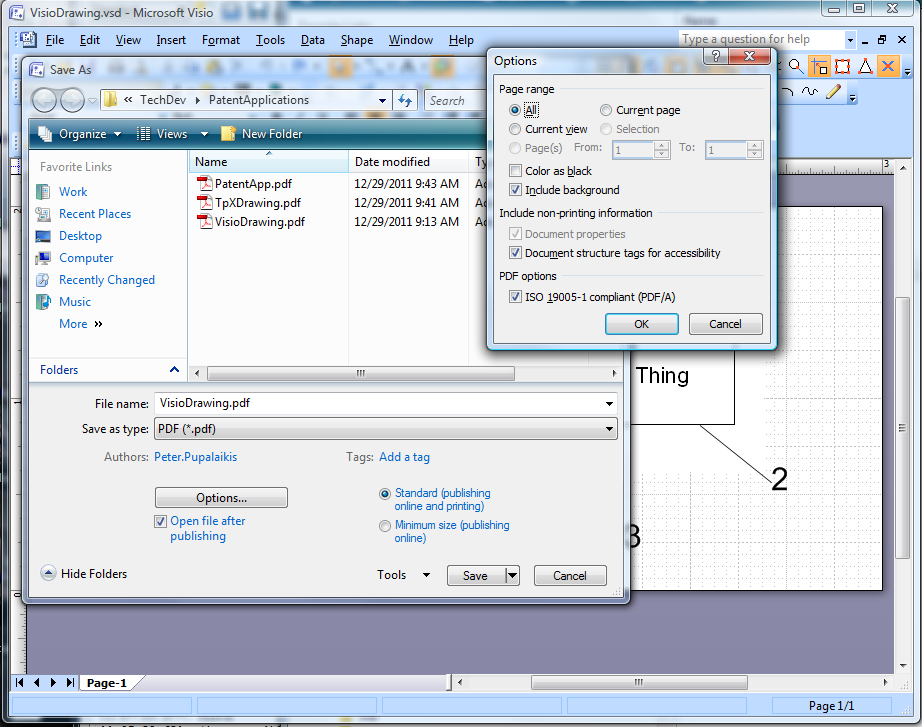
\includegraphics[scale=0.4]{VisioSave}
\par\end{centering}

\caption{Saving Visio Drawings as PDF}
\label{fig:AccessTpXDrawingProperties-1}\index{PDF}
\end{figure}
When editing and saving your Visio drawing, you'll want to save your
drawing in Visio format and save it as a PDF. The PDF document is
what gets included in the application. To do this, you want to use
{[}Save As...{]}, select PDF\index{PDF} as the type, then make sure
the options are set to ISO 19005-1 compliant PDF.


\subsection{TpX\label{sub:TpX}}

TpX\index{TpX} is the best tool for creating \LaTeX{} drawings. What's
good about it is that it easily allows importing other documents and
touching them up. More importantly though, it allows automatic drawing
annotation. This section will explain what you need to know to deal
with TpX documents.


\subsubsection{TpX Settings\label{sub:TpX-Settings}}

Your TpX\index{TpX!settings} document must be saved with certain
settings. These settings can be found under the menu {[}Edit{]}{[}Picture
properties{]} as shown in \figref{AccessTpXDrawingProperties}.
\begin{figure}
\begin{centering}
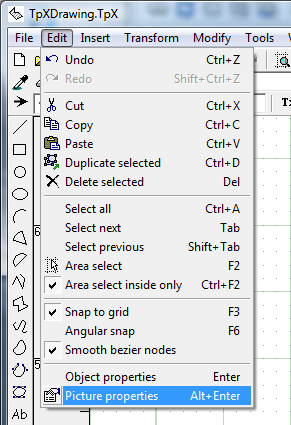
\includegraphics[scale=0.5]{TpXSettingsAccess}
\par\end{centering}

\caption{Accessing TpX Drawing Properties}
\label{fig:AccessTpXDrawingProperties}
\end{figure}


You will only need to change a few very important properties. These
are:
\begin{itemize}
\item \setlength{\itemsep}{0mm} \TeX{}Format=none - this prevents writing
out spurious EPS files.
\item Pdf\TeX{}Format=pdf\index{PDF} or tikz\index{TikZ} (recommended)
- this causes the graphics portion of the drawing to be output in
PDF if pdf is selected or it is embedded within the TpX document in
\TikZ~ format if tikz is chosen.
\item \TeX{}Figure=none - this prevents the \LaTeX{} portion of the file
from including figure information which is already included in the
macro that imports the file.
\item FontSizeIn\TeX{}=0 - this causes the font size to be used from your
patent application document settings.
\end{itemize}
A comprehensive list of the desired settings are:
\begin{itemize}
\item \setlength{\itemsep}{0mm} Caption=
\item Comment=
\item Label=
\item PicScale=1
\item Border=2
\item \TeX{}Format=none
\item Pdf\TeX{}Format=pdf\index{PDF} or tikz\index{TikZ} (recommended)
\item BitmapRes=20000
\item PicMagnif=1
\item IncludePath=
\item LineWidth=0.3
\item ArrowsSize=0.7
\item StarsSize=1
\item HatchingStep=2
\item HatchingLineWidth=0.5
\item DottedSize=0.5
\item DashSize=1
\item DefaultFontHeight=5
\item FontName=
\item DefaultSymbolSize=30
\item ApproximationPrecision=0.01
\item MiterLimit=10
\item \TeX{}CenterFigure=1
\item \TeX{}Figure=none
\item \TeX{}FigurePlacement=
\item \TeX{}FigurePrologue=
\item \TeX{}FigureEpilogue=
\item \TeX{}PicEpilogue=
\item FontSizeIn\TeX{}=0
\item MetaPost\TeX{}Text=1
\end{itemize}

\subsubsection{Drawing Size}

\index{figure!size}\index{TpX!figure size}Unfortunately (for Americans),
TpX operates with grids that are metric only. TpX drawings are absolutely
sized with the origin at 0,0 in the lower left corner. The numbering
of the grids is in millimeters. You will want to make sure your drawing
is no larger than $6^{"}\times9^{"}$ which means 150 mm $\times$
230 mm. Remember, you will need to place annotation lines outside
the drawing, so ideally, you want to keep the drawing without annotations
to $5^{"}\times8^{"}$ which means 130 mm $\times$ 200 mm. Usually,
I place a rectangle filled white set to the back with white lines
(i.e. no lines showing) first that are the exact size I want the drawing
to be so that I don't go outside the boundaries.


\subsubsection{Annotations\label{sub:Annotations-1}}

\index{annotation!in TpX}\index{TpX!annotations}TpX is great for
annotating because it can be handled automatically. This is done by
drawing a line to the element and then labeling it. The line drawing
is self explanatory. The labeling should be such that it is aligned
1 mm below the line end vertically and lined up with the line end
horizontally as shown in \figref{AnnotationAlignment}.

\begin{figure}
\centering{}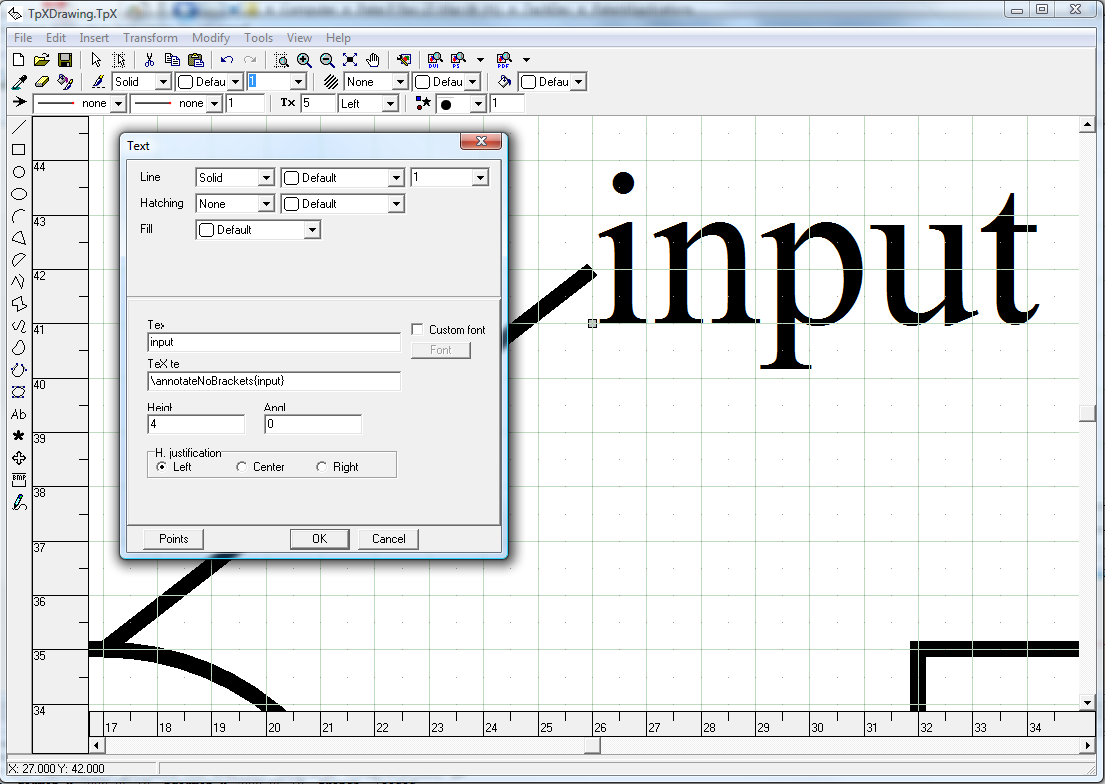
\includegraphics[scale=0.4]{annotationAlignment}\caption{Annotation Alignment}
\label{fig:AnnotationAlignment}\index{annotation!in TpX}\index{TpX!annotations}
\end{figure}
Notice in \figref{AnnotationAlignment} that the text properties dialog
is shown showing how the annotation is labeled. TpX enables two types
of annotation labels:
\begin{itemize}
\item \TeX{} - the text you will see on the diagram which can be labeled
in plain English. This text will not actually show up in your figure
if there is a Tex te label.
\item \TeX{} te - the text that describes what will be seen in the diagram.
Note here that we use the \index{annotationNumberReference macro@\textbackslash{}annotationNumberReference macro}\index{LaTeX@\LaTeX{}!macro!annotationNumberReference@\textbackslash{}annotationNumberReference}\index{annotateNoBrackets macro@\textbackslash{}annotateNoBrackets macro}\index{LaTeX@\LaTeX{}!macro!annotateNoBrackets@\textbackslash{}annotateNoBrackets}macro
\textbackslash{}annotateNoBrackets\{input\} which tells the document
compiler to figure out the number that belongs in the label. In order
for this to work properly, the label input must have been entered
in the annotation list as described in \secref{Drawings}. If you
don't, the drawing will show ?? for the number when you print your
application. 
\end{itemize}
As mentioned, these text labels can be used in two ways:
\begin{itemize}
\item no \TeX{} te label - the label shown in the drawing and in your document
will be the label shown in the \TeX{} box.
\item \TeX{} te label provided - the label shown while editing your document
will be the \TeX{} label, but the label shown when you print your
document will be the \TeX{} te label which can be a macro, if desired.
\end{itemize}
If using TpX, you should know that the size of the drawing will be
such that a box can surround the figure, as seen on the TpX screen.
This means according to the \TeX{} text shown, which is unfortunate.
You will need to keep your \TeX{} text short so that it does not make
TpX think that the drawing is larger than it will actually be when
formatted.


\subsubsection{Text Labels}

Text labels may be added to your drawing by using insert text. When
you insert text, there are many possibilities for how your text labels
will be shown. You can use macros, formulas and other things as well
as plain text. The strategy you want to follow is when you are inserting
just plain text, then use insert text and just type it in. When you
are inserting something other than plain text, like a formula, then
use insert text, type in some text that you want to see when editing
the document (you cannot see the actual formula until you view the
final document), and then edit the text properties. When you edit
the text properties, you will see two boxes as shown in \figref{AnnotationAlignment}:
\begin{itemize}
\item \TeX{} - the text you will see on the diagram which can be labeled
in plain English. This text will not actually show up in your figure
if there is a Tex te label.
\item \TeX{} te - the text that describes what will be seen in the final
output. This can be plain text, \LaTeX{} formulas, macros, etc. The
writing of \LaTeX{} formulas is beyond the scope of this document.
Just know that you have this capability.
\end{itemize}
\cleartooddpage
\renewcommand{\sectionmark}[1]{\markright{#1}}

\cleardoublepage{}


\section*{Appendix A - uspatent.cls Listing}

\addcontentsline{toc}{section}{Appendix A - uspatent.cls Listing}
\sectionmark{Appendix A - uspatent.cls Listing}
\begin{lstlisting}
%%
%% This is file `uspatent.cls',
%% 
%% 
%%   Author: Peter J. Pupalaikis  (pete_pope  at hotmail dot com)
%%   Copyright 2012 Peter J. Pupalaikis
%%   Version 1.0
%% 
%%   This work may be distributed and/or modified under the
%%   conditions of the LaTeX Project Public License, either
%%   version 1.3 of this license or (at your option) any
%%   later version.
%%   The latest version of the license is in
%%      http://www.latex-project.org/lppl.txt
%%   and version 1.3 or later is part of all distributions of
%%   LaTeX version 2003/06/01 or later.
%% 
%%   This work consists of the files listed in the README file.
%% 
\NeedsTeXFormat{LaTeX2e}
\ProvidesClass{uspatent}%
  [2012/06/09 v0.0 U.S. Patent Application Class]
%\DeclareOption*{\PassOptionsToClass{\CurrentOption}{memoir}}
%\ProcessOptions
\LoadClass[letterpaper,12pt]{memoir}[1996/10/24]

\newif\ifPatentOfficeMode
\PatentOfficeModetrue

\newcommand{\setAssigneeName}{\def\assigneeName}
\newcommand{\setAssigneeAddress}{\def\assigneeAddress}
\newcommand{\setAssigneeCity}{\def\assigneeCity}
\newcommand{\setAssigneePhone}{\def\assigneePhone}
\newcommand{\setDocketNumber}{\def\patentNumber}
\newcommand{\setLawyerName}{\def\patentLawyerName}
\newcommand{\setLawyerNumber}{\def\patentLawyerNumber}
\newcommand{\setLawyerPhone}{\def\patentLawyerPhone}
\newcommand{\setOtherInventor}[1]{\otherInventor{#1}}
\newcommand{\setDocumentVersion}{\def\patentDocumentVersion}
\newcommand{\setPrintingModeDraft}{\PatentOfficeModefalse}
\newcommand{\setPrintingModeApplication}{\PatentOfficeModetrue}
\newcommand{\inventor}{\author}

\settrimmedsize{11in}{8.5in}{*}
\setlength{\trimtop}{0pt}
\setlength{\trimedge}{0pt}
\settypeblocksize{8.5in}{36pc}{*}
\setulmargins{1.5in}{*}{*}
\setlrmargins{*}{*}{1}
\setmarginnotes{17pt}{51pt}{\onelineskip}
\setheadfoot{5\onelineskip}{3\onelineskip}
\setheaderspaces{*}{2\onelineskip}{*}
\checkandfixthelayout
\captiondelim{}

\ifpdf
\usepackage[pdftex]{graphicx}
%No Commas in the PDF Title!?!
\usepackage[
hyperindex=true,
pdfusetitle,
bookmarks=true,
extension= pdf,
linkcolor=black,
colorlinks=true,
hyperfootnotes=false,
pdffitwindow=true,
pdftoolbar=true,
pdfmenubar=true,
debug=false,
pagebackref=true
]{hyperref}
\DeclareGraphicsExtensions{ .pdf, .jpg, .tif}
\else
\usepackage[dvips]{graphicx}
\DeclareGraphicsExtensions{ .eps, .jpg }
\fi

\usepackage{amsmath}
\usepackage{enumitem}
\usepackage[nolist]{acronym}
\usepackage{memhfixc}
\usepackage{xspace}
\usepackage{prettyref}
\usepackage{lmodern}
\usepackage[T1]{fontenc}
\usepackage{babel}
\usepackage{tikz}

\newrefformat{eq}{\textup{(\ref{#1})}}
\newrefformat{cla}{claim \ref{#1}}
\newrefformat{tab}{Table \ref{#1}}
\newrefformat{fig}{\figurename \ \textbf{\ref{#1}}}

\newcommand{\patentTitlePage}{%

\ifx\assigneeName\undefined
\global\edef\assigneeName{~}
\global\edef\confidentialAssignee{~}
\else
\global\edef\confidentialAssignee{%
Confidential Property of \assigneeName}
\fi
\ifx\assigneeAddress\undefined
\global\edef\assigneeAddress{~}
\fi
\ifx\assigneeCity\undefined
\global\edef\assigneeCity{~}
\fi
\ifx\assigneePhone\undefined
\global\edef\assigneePhone{~}
\fi
\ifx\patentNumber\undefined
\global\edef\patentNumber{~}
\fi
\ifx\patentLawyerName\undefined
\global\edef\patentLawyerName{~}
\fi
\ifx\patentLawyerNumber\undefined
\global\edef\patentLawyerNumber{~}
\fi
\ifx\patentLawyerPhone\undefined
\global\edef\patentLawyerPhone{~}
\fi
\ifx\patentDocumentVersion\undefined
\global\edef\patentDocumentVersion{0.0}
\fi
\ifx\thedate\undefined
\global\edef\thedate{\today}
\fi

\ifPatentOfficeMode
%patent office mode
\pagestyle{title}
\makeoddhead{myheadings}
{}{}{\scriptsize{\patentNumber}}
\makeevenhead{myheadings}
{}{}{\scriptsize{\patentNumber}}
\else
%not patent office mode
\pagestyle{title}
\makeoddhead{myheadings}
{\confidentialAssignee}
{}
{\scriptsize{Draft of \thedate\\version \patentDocumentVersion}}
\makeevenhead{myheadings}
{\confidentialAssignee}
{}
{\scriptsize{Draft of \thedate\\version \patentDocumentVersion}}
\fi
\begin{titlingpage}
\aliaspagestyle{titlingpage}{myheadings}
\begin{center}
\textbf{APPLICATION FOR UNITED STATES LETTERS PATENT} 
\vskip 172 pt
Title: \MakeUppercase{ \thetitle } 
\end{center}
\vskip 172 pt
\begin{flushleft} \begin{tabular}{rl}  Inventors:  & 
\theauthor \\
& \inventorListName{1} \\
& \inventorListName{2} \\
& \inventorListName{3} \\
& \inventorListName{4} \\
& \inventorListName{5} \\
& \inventorListName{6} \\
& \inventorListName{7} \\
& \inventorListName{8} \\
\end{tabular}\par \end{flushleft}
\begin{flushright}
\tiny{
\vskip 10 pt
%\\[4\baselineskip]
\patentLawyerName \\
\patentLawyerNumber \\
[2\baselineskip]
\assigneeName \\
\assigneeAddress \\
\assigneeCity \\
\assigneePhone
}
\end{flushright}
\end{titlingpage}
\parindent 10pt
\DoubleSpacing
}

\renewcommand{\maketitle}{
\patentTitlePage
\patentStart
}

\def\figureName{FIG.}

\def\etal{%
\expandafter\ifx\csname inventorname 1\endcsname\relax
\else
~et~al.
\fi
}

% use this command to put a comment in the margin
\newcommand{\patentComment}[1]{
\ifPatentOfficeMode
%patent office mode
\else
%not patent office mode
\begin{SingleSpace}
\marginpar{\tiny\textcolor{red}{ \begin{flushleft} #1 \end{flushleft}}}
\end{SingleSpace}
\fi
}

\newcommand{\patentSection}[1]{
\Needspace{8pc}
\section[#1][]{}
%\label{#2}
\begin{center}
\textbf{\underline{\MakeUppercase{{#1}}}}
\end{center}
}

\newcommand{\patentParagraph}{
\par\noindent
\refstepcounter{parnum}[\textbf{%
\ifnum \value{parnum} < 10 0\else\fi
\ifnum \value{parnum} < 100 0\else\fi
\ifnum \value{parnum} < 1000 0\else\fi
\arabic{parnum}}]
\indent}

\newcommand{\patentStart}{
\ifPatentOfficeMode
%patent office mode
\pagestyle{myheadings}
\makeoddhead{myheadings}{}{}{\scriptsize{\patentNumber}}
\makeevenhead{myheadings}{}{}{\scriptsize{\patentNumber}}
\makeoddfoot{myheadings}{}{\thepage}{}
\makeevenfoot{myheadings}{}{\thepage}{}
\else
%not patent office mode
\pagestyle{myheadings}
\makeoddhead{myheadings}
{\confidentialAssignee}
{}{\scriptsize{Draft of \thedate\\version \patentDocumentVersion}}
\makeevenhead{myheadings}
{\confidentialAssignee}
{}{\scriptsize{Draft of \thedate\\version \patentDocumentVersion}}
\makeoddfoot{myheadings}{\thepage}{}{\scshape{\tiny{\thetitle}}}
\makeevenfoot{myheadings}{\scshape{\tiny{\thetitle}}}{}{\thepage}
\fi

\begin{center}\textbf{\MakeUppercase{ \thetitle }}\end{center}

% don't show section numbers!
\setcounter{secnumdepth}{-1}
% let them go into the "TOC" (even though we won't print it) because
% this allows the PDF file to contain the appropriate bookmarks
\setcounter{tocdepth}{1}

\setbeforesecskip{0pc}
\setaftersecskip{0pc}
\parskip=10pt

% this is used to number paragraphs
\newcounter{parnum}
}


\makeatletter
\newcount\@inventornumber
\@inventornumber=0
\makeatother

\makeatletter
\def\otherInventor#1{
\global\advance\@inventornumber by 1
\expandafter\edef\csname inventorname \the\@inventornumber\endcsname{#1}}
\makeatother

\def\inventorListName#1{\csname inventorname #1\endcsname}

% Claims are the only area where I still use labels, hence the
% prettyref include.
% \patentClaimsStart essentially begins the enumerate environment and 
% \patentClaimsEnd essentially ends it.
% I'd like to remove this dependency someday and use the counter
% mechanisms used elsewhere.

% Inside, a claim is begin with \beginClaim which labels it and starts
% an \item.
% Claims are referenced with \claimRef
\newcommand{\beginClaim}[1]{\item \label{cla:#1}}
\newcommand{\claimRef}[1]{claim \ref{cla:#1}}

\newcommand{\WhatIsClaimed}{What is claimed:}

\newcommand{\patentClaimsStart}{
\newpage
\section[Claims][]{}
\parskip=0pt
\WhatIsClaimed
\begin{enumerate}
}

\newcommand{\patentClaimsEnd}{
\end{enumerate}
\newpage
}

%I'm not sure what this is but I'm afraid to remove it
\newcommand{\putfigcaption}{}

% Patent drawings have a special header that numbers the drawing pages
\newcommand{\patentDrawingsStart}{
\cleartooddpage
%\newpage
\ifPatentOfficeMode
%patent office mode
\setcounter{page}{1}
\pagestyle{myheadings}
\makeoddhead{myheadings}{}{
\tiny{\thetitle} \\
\tiny{\theauthor\etal} \\
\tiny{\patentNumber} \\
\tiny{\patentLawyerName\ \patentLawyerPhone}\\[.1in]
\tiny{\thepage/\thelastpage}
}{}
\makeevenhead{myheadings}{}{
\tiny{\thetitle} \\
\tiny{\theauthor\etal} \\
\tiny{\patentNumber} \\
\tiny{\patentLawyerName\ \patentLawyerPhone}\\[.1in]
\tiny{\thepage/\thelastpage}
}{}
\makeoddfoot{myheadings}{}{}{}
\makeevenfoot{myheadings}{}{}{}
\else
%not patent office mode
\pagestyle{myheadings}
\makeoddhead{myheadings}
{\confidentialAssignee}
{}
{\scriptsize{Draft of \thedate\\version \patentDocumentVersion}}
\makeevenhead{myheadings}
{\confidentialAssignee}
{}
{\scriptsize{Draft of \thedate\\version \patentDocumentVersion}}
\makeoddfoot{myheadings}{\thepage}{}{\scshape{\tiny{\thetitle}}}
\makeevenfoot{myheadings}{\scshape{\tiny{\thetitle}}}{}{\thepage}
\fi

\section[Drawings][]{}
\begin{SingleSpace}
}

\newcommand{\patentDrawingsEnd}{
\end{SingleSpace}
%\newpage
\clearpage
}

\makeatletter
\newcount\@annotationnumber
\@annotationnumber=0
\makeatother

\makeatletter
\newcount\@annotationfigurenumber
\@annotationfigurenumber=0
\makeatother

\makeatletter
\def\advanceannotationfigurenumber{
\global\advance\@annotationfigurenumber by 1}
\makeatother

\makeatletter
\def\setannotationnumber#1{%
\global\@annotationnumber=#1
\global\advance\@annotationnumber by -1
}
\makeatother

\def\annotationnextfigure{
\global\advance\@annotationfigurenumber by 1}

\makeatletter
\def\setannotationfigurenumber#1{%
\global\@annotationfigurenumber=#1
}
\makeatother

\makeatletter
\def\@newannotation#1{
\expandafter\ifx\csname anonum#1 \endcsname\relax
\global\advance\@annotationnumber by 1
\expandafter\edef\csname anoele \the\@annotationnumber\endcsname{#1}
\expandafter\edef\csname anonum#1 \endcsname{\the\@annotationnumber}
\expandafter\edef\csname anofignum \the\@annotationnumber\endcsname{%
\the\@annotationfigurenumber}
\else\message{error: duplicate annotation #1}\fi}
\makeatother

\makeatletter
\def\annotationDefinition{%
\@ifnextchar[{\@annotationDefinitionmulti}{\@newannotation}}
\def\@annotationDefinitionmulti[#1]#2{%
\@newannotation{#2}\annotationName{#1}
\@ifnextchar[{\@annotationDefinitionfull}{}}
\def\@annotationDefinitionfull[#1]{\annotationDescription{#1}}
\makeatother

\makeatletter
\def\annotationDescription#1{%
\expandafter\ifx\csname anodesc \the\@annotationnumber\endcsname\relax
\expandafter\def\csname anodesc \the\@annotationnumber\endcsname{#1}
\else
\message{error while assigning description ``#1'' to annotation variable
``\annotationListVariableName{\the\@annotationnumber}''
 - it was already defined as
``\annotationListDescription{\the\@annotationnumber}''.}\fi}
\makeatother

\makeatletter
\def\annotationName#1{%
\expandafter\ifx\csname anotext \the\@annotationnumber\endcsname\relax
\expandafter\def\csname anotext \the\@annotationnumber\endcsname{#1}
\else
\message{error while assigning text name ``#1'' to annotation variable
``\annotationListVariableName{\the\@annotationnumber}''
 - it was already defined as
``\annotationListText{\the\@annotationnumber}''.}\fi}
\makeatother

\makeatletter
\def\annotationReference#1{%
[\thinspace\annotationNumberReference{#1}\thinspace]}
\makeatother

\def\annotationNameAndReference#1{%
\annotationTextReference{#1}~\annotationReference{#1}}

\def\annotationDescriptionreference#1{%
\csname anodesc \annotationNumberReference{#1}\endcsname}

\def\annotationTextReference#1{%
\csname anotext \annotationNumberReference{#1}\endcsname}

\def\annotationNumberReference#1{\csname anonum#1 \endcsname}

\def\annotationNumberReferenceUnderlined#1{\underline{\csname anonum#1 \endcsname}}

\def\annotationListVariableName#1{\csname anoele #1\endcsname}

\def\annotationListText#1{\csname anotext #1\endcsname}

\def\annotationListDescription#1{\csname anodesc #1\endcsname}

\def\annotationListFigureNumber#1{\csname anofignum #1\endcsname}

\def\annotationListFigureDescription#1{\csname anofigdesc #1\endcsname}

\def\annotationListFigureExtension#1{\csname anofigext #1\endcsname}

\def\annotationListFigureCaption#1{\csname anofigcap #1\endcsname}

\def\annotationListFigureName#1{\csname anofigname #1\endcsname}

\def\annotationListPrintFigure#1#2{
\edef\testa{#1}\edef\testb{#2}\edef\testzero{0}
\ifx\testb\testzero
\figureName #1---\annotationListFigureName{#1}.%
\annotationListFigureExtension{#1}%
---\annotationListFigureDescription{#1}
\par
\else
\ifx\testa\testb
\else
\figureName #1---\annotationListFigureName{#1}.%
\annotationListFigureExtension{#1}%
---\annotationListFigureDescription{#1}
\par
\fi\fi
}

\def\annotationListSectionName{\section*{Annotation List}}

\makeatletter
\def\printAnnotationList{{%
\@annotationnumber=1
\@annotationfigurenumber=0
\expandafter\ifx\csname anoele \the\@annotationnumber\endcsname\relax
\else
\annotationListSectionName\par
\loop
\expandafter\ifx\csname anoele \the\@annotationnumber\endcsname\relax
\else
\leftskip = -10 pt
\annotationListPrintFigure{%
\annotationListFigureNumber{\the\@annotationnumber}}
{\the\@annotationfigurenumber}
\leftskip = 10 pt
%\hangindent = 20 pt
%\hangafter
\par
\@annotationfigurenumber=%
\annotationListFigureNumber{\the\@annotationnumber}
\the\@annotationnumber---%
\annotationListVariableName{\the\@annotationnumber}---%
\annotationListText{\the\@annotationnumber}---%
\annotationListDescription{\the\@annotationnumber}
\par
\leftskip = -10 pt
\advance\@annotationnumber by 1
\repeat
\fi
}}
\makeatother

\def\annotationFigureListPrintFigure#1{
\figureName ~#1 \annotationListFigureDescription{#1}}

\def\annotationFigureListSectionName{%
\section*{Brief Description of the Drawings}}
\def\annotationFigureListPreamble{%
For a more complete understanding of the invention,
reference is made to the following description and accompanying
drawings, in which:\par}

\def\setFigureListNoRunOn{%
\def\annotationFigureListLast{.}
\def\annotationFigureListNextLast{.}
\def\annotationFigureListOther{.}
}

\def\annotationFigureListLast{.}
\def\annotationFigureListNextLast{; and}
\def\annotationFigureListOther{;}

\makeatletter
\def\printAnnotationFigureList{{
\@annotationfigurenumber=1
\expandafter\ifx\csname anofigdesc \the\@annotationfigurenumber\endcsname\relax
\else
\annotationFigureListSectionName\par
\annotationFigureListPreamble\par
\loop
\expandafter\ifx\csname anofigdesc \the\@annotationfigurenumber\endcsname\relax
\else
\annotationFigureListPrintFigure{\the\@annotationfigurenumber}%
{\advance\@annotationfigurenumber by 1
\expandafter\ifx\csname anofigdesc \the\@annotationfigurenumber\endcsname\relax
\annotationFigureListLast\else{\advance\@annotationfigurenumber by 1
\expandafter\ifx\csname anofigdesc \the\@annotationfigurenumber\endcsname\relax
\annotationFigureListNextLast\else\annotationFigureListOther\par\fi}\fi}
\advance\@annotationfigurenumber by 1
\repeat
\fi
}}
\makeatother

\makeatletter
\def\figureDescription#1{%
\expandafter\ifx\csname anofigdesc \the\@annotationfigurenumber\endcsname\relax
\expandafter\def\csname anofigdesc \the\@annotationfigurenumber\endcsname{#1}
\else
\message{error while assigning description ``#1'' to annotation figure number
``\the\@annotationfigurenumber'' - it was already defined as
``\annotationListFigureDescription{\the\@annotationfigurenumber}''.}\fi}
\makeatother

\makeatletter
\def\figureExtension#1{%
\expandafter\ifx\csname anofigext \the\@annotationfigurenumber\endcsname\relax
\expandafter\def\csname anofigext \the\@annotationfigurenumber\endcsname{#1}
\else
\message{error while assigning extension ``#1'' to annotation figure number
``\the\@annotationfigurenumber'' - it was already defined as
``\annotationListFigureExtension{\the\@annotationfigurenumber}''.}\fi}
\makeatother

\makeatletter
\def\figureCaption#1{%
\expandafter\ifx\csname anofigcap \the\@annotationfigurenumber\endcsname\relax
\expandafter\def\csname anofigcap \the\@annotationfigurenumber\endcsname{#1}
\else
\message{error while assigning caption ``#1'' to annotation figure number 
``\the\@annotationfigurenumber'' - it was already defined as
``\annotationListFigureCaption{\the\@annotationfigurenumber}''.}\fi}
\makeatother

\makeatletter
\def\figureClearPageAfter{%
\expandafter\def\csname anofigcp \the\@annotationfigurenumber\endcsname{}}
\makeatother

\makeatletter
\def\@newfigure#1{
\expandafter\ifx\csname fignum#1 \endcsname\relax
\global\advance\@annotationfigurenumber by 1
\expandafter\edef\csname anofigname \the\@annotationfigurenumber\endcsname{#1}
\expandafter\edef\csname fignum#1 \endcsname{\the\@annotationfigurenumber}
\else\message{error: duplicate annotation #1}\fi}
\makeatother

\makeatletter
\def\figureDefinition{\@ifnextchar[{\@figuredefinitionmulti}{\@newfigure}}
\def\@figuredefinitionmulti[#1]#2{\@newfigure{#2}\figureDescription{#1}}
\makeatother

\makeatletter
\def\figureReference#1{FIG.~\figurenumberreference{#1}}
\makeatother

\def\figurenumberreference#1{\csname fignum#1 \endcsname}

\expandafter\def\csname showfigure pdf\endcsname #1#2#3{%
\begin{figure}[!ht]
\centering
\includegraphics[]{#1.#2}\par
\figureReference{#1}~~#3 \par
\end{figure}
}

\expandafter\def\csname showfigure tpx\endcsname #1#2#3{%
\begin{figure}[ht]
\centering
\input{"#1.tpx"}\par
\figureReference{#1}~~#3 \par
\end{figure}
}

\expandafter\def\csname showfigure tex\endcsname #1#2#3{%
\begin{figure}[ht]
\centering
\input{"#1.tex"}\par
\figureReference{#1}~~#3 \par
\end{figure}
}

\expandafter\def\csname showfigure placeholder\endcsname #1#2#3{%
\begin{figure}[ht]
\centering
no extension provided for file name #1.\par This will be
used as a placeholder\par
\figureReference{#1}~~#3 \par
\end{figure}
}

\expandafter\def\csname showfigure unk\endcsname #1#2#3{%
\begin{figure}[ht]
\centering
\includegraphics[]{#1.#2}\par
\figureReference{#1}~~#3 \par
\end{figure}
}

\makeatletter
\def\figures{{%
\@annotationfigurenumber=1
\expandafter\ifx\csname anofigname \the\@annotationfigurenumber\endcsname\relax
\else
\figuresStart
\loop
\expandafter\ifx\csname anofigname \the\@annotationfigurenumber\endcsname\relax
\else
\expandafter\ifx\csname anofigext \the\@annotationfigurenumber\endcsname\relax
\edef\figureextension{placeholder}
\else
\edef\figureextension{%
\annotationListFigureExtension{\the\@annotationfigurenumber}}
\fi
\expandafter\ifx\csname showfigure \figureextension\endcsname\relax
% this is an unknown figure extension
\def\figureshower{\csname showfigure unk\endcsname}
\else
\def\figureshower{\csname showfigure \figureextension\endcsname}
\fi
\figureshower{\annotationListFigureName{\the\@annotationfigurenumber}}%
{\figureextension}%
{\annotationListFigureCaption{\the\@annotationfigurenumber}}
\expandafter\ifx\csname anofigcp \the\@annotationfigurenumber\endcsname\relax
\else
\clearpage
\fi
\advance\@annotationfigurenumber by 1
\repeat
\figuresEnd
\fi
}}
\makeatother

\def\annotationFigureListSectionName{
\patentSection{Brief Description of the Drawings}}

\def\annotationListSectionName{\patentSection{Annotation List}}

\def\annotationFigureListPreamble{
\patentParagraph{For a more complete understanding of the invention,
reference is made to the following description and accompanying
drawings, in which:}}

\def\patentDrawingDescriptions{\printAnnotationFigureList}

\def\referencePatentFigure#1{\figureReference{#1}}
\def\annotate#1{\annotationReference{#1}}
\def\annotateWithName#1{\annotationNameAndReference{#1}}

\def\annotationFigureListPrintFigure#1{
\patentParagraph{\figureName ~#1 is \annotationListFigureDescription{#1}}}

\def\annotateNoBrackets#1{\annotationNumberReference{#1}}

\def\figuresStart{\patentDrawingsStart}
\def\figuresEnd{\patentDrawingsEnd}

\def\patentDrawings{%
\ifPatentOfficeMode
\else
\printAnnotationList
\fi

\figures
}

\endinput
%%
%% End of file `patent.cls'.
\end{lstlisting}


\cleartooddpage

\cleardoublepage{}


\section*{Appendix B - PatentLayout.tex Listing }

\noindent \begin{flushleft}
\addcontentsline{toc}{section}{Appendix B - PatentLayout.tex Listing}
\sectionmark{Appendix B - PatentLayout.tex Listing} 
\begin{lstlisting}
%%
%% This is file `PatentApplication.tex',
%% 
%% 
%%   Author: Peter J. Pupalaikis  (pete_pope  at hotmail dot com)
%%   Copyright 2012 Peter J. Pupalaikis
%%   Version 1.0
%% 
%%   This work may be distributed and/or modified under the
%%   conditions of the LaTeX Project Public License, either
%%   version 1.3 of this license or (at your option) any
%%   later version.
%%   The latest version of the license is in
%%      http://www.latex-project.org/lppl.txt
%%   and version 1.3 or later is part of all distributions of
%%   LaTeX version 2003/06/01 or later.
%% 
%%   This work consists of the files listed in the README file.
%% 
\documentclass[english]{uspatent}
\begin{document}

\setAssigneeName{Assignee Name}
\setAssigneeAddress{Assignee Address}
\setAssigneeCity{Assignee City, State, Zip}
\setAssigneePhone{Assignee Phone}
\setDocketNumber{Docket Number}
\setLawyerName{Patent Lawyer Name}
\setLawyerNumber{Patent Lawer Reg. Number}
\setLawyerPhone{Patent Lawyer Phone}
\setOtherInventor{Another Inventor}
\setOtherInventor{Yet Another Inventor}
\setDocumentVersion{0.0}
\setPrintingModeApplication

\figureDefinition{VisioDrawing}
\figureExtension{pdf}
\figureDescription{is an example drawing created in Visio}

\annotationDefinition{Widget}
\annotationName{widget}
\annotationDescription{a widget in the Visio drawing}
\annotationDefinition{Thing}
\annotationName{thing}
\annotationDescription{a thing in the visio drawing}
\annotationDefinition{WidgetThingConnection}
\annotationName{connection}
\annotationDescription{the arrow connecting the widget and the thing}

\figureDefinition{TpXDrawing}
\figureExtension{tpx}
\figureCaption{PRIOR ART}
\figureDescription{is an example drawing created in TpX}

\annotationDefinition{input}
\annotationName{input}
\annotationDescription{the input}
\annotationDefinition{output}
\annotationName{output}
\annotationDescription{the output}
\annotationDefinition{mathProcessor}
\annotationName{math processor}
\annotationDescription{the math procesor}


\title{Invention Name Not Yet Defined}
\date{Date of this version}
\inventor{First Named Inventor}

\maketitle

\patentSection{Field of the Invention}

\patentParagraph Describe the field of the invention like...

\patentParagraph The present invention relates to \ldots and in particular to \ldots

\patentParagraph In other words, the basic types of things that the invention improves or is implemented in.

\patentSection{Background of the Invention}

\patentParagraph Describe the past. Focus on problems that you will be solving. Talk about prior-art in detail to describe what has been done before and what the problems are. You are telling a story that inevitably leads up to ending statements like:

\patentParagraph What is needed is\ldots

\patentParagraph The things that are needed will be put forth as solutions in the next section.

\patentSection{Objects of the Invention}

\patentParagraph It is an object of this invention to \ldots Note that the objects should match the things that are needed as described in the last section. Do not describe the invention here, just the problems that will be solved or the utility of the invention.

\patentParagraph Still other objects and advantages of the invention will in part be obvious and will in part be apparent from the specification and drawings.

\patentSection{Summary of the Invention}

\patentParagraph In order to overcome \ldots, we do\ldots

\patentParagraph The invention accordingly comprises the several steps and the relation of one or more of such steps with respect to each of the others, and the apparatus embodying features of construction, combinations of elements and arrangement of parts that are adapted to affect such steps, all is exemplified in the following detailed disclosure, and the scope of the invention will be indicated in the claims.

\patentDrawingDescriptions

\patentSection{Detailed Description of the Preferred Embodiments}

\patentParagraph The details of the invention go here. I will use this area to make reference to the drawings so you can see how it's done.

\patentParagraph The arrangement in \referencePatentFigure{VisioDrawing} shows an exemplary arrangement of a preferred embodiment. In \referencePatentFigure{VisioDrawing}, one sees a \annotateWithName{Widget} and a \annotateWithName{Thing} with a preferable \annotateWithName{WidgetThingConnection} that enables the \annotateWithName{Thing} to process the data coming from the \annotateWithName{Widget}. I think you get the idea.  You can refer to the number as \annotationNumberReferenceUnderlined{Widget}.

\patentParagraph You can either write: \annotateWithName{Thing} or you can write thing~\annotate{Thing}. They both produce the same thing.

\patentParagraph Note that you make and refer to equations like this:

\begin{equation}
E=mc^{2}\label{eq:energy}
\end{equation}

\patentParagraph One of my favorite equations is:

\begin{equation}
e^{j\theta}=\cos\left(\theta\right)+j\cdot\sin\left(\theta\right)\label{eq:euler}
\end{equation}

\patentParagraph We refer to the first equation as \prettyref{eq:energy} and the second as \prettyref{eq:euler}. The second equation \prettyref{eq:euler} is Euler's equation.

\patentParagraph It will thus be seen that the objects set forth above, among those made apparent from the preceding description, are efficiently attained and, because certain changes may be made in carrying out the above method and in the construction(s) set forth without departing from the spirit and scope of the invention, it is intended that all matter contained in the above description and shown in the accompanying drawings shall be interpreted as illustrative and not in a limiting sense.

\patentParagraph It is also to be understood that the following claims are intended to cover all of the generic and specific features of the invention herein described and all statements of the scope of the invention which, as a matter of language, might be said to fall therebetween.

\patentClaimsStart

\beginClaim{Claim1}

This is an independent claim.

\beginClaim{Claim2}

The method of \claimRef{Claim1} further comprising\ldots

\patentClaimsEnd

\patentSection{Abstract}

A simple statement of what the invention pertains to\ldots

\patentDrawings
\end{document}
\end{lstlisting}

\par\end{flushleft}

\cleardoublepage{}

\cleartoevenpage


\section*{Appendix C - Patent Application Document Printout}

\addcontentsline{toc}{section}{Appendix C - Patent Application Document Printout}
\sectionmark{Appendix C - Patent Application Document Printout}The following pages contain a printout of the final document created
upon compilation of the PatentApplication.lyx or PatentApplication.tex
document with the uspatent.cls file provided.

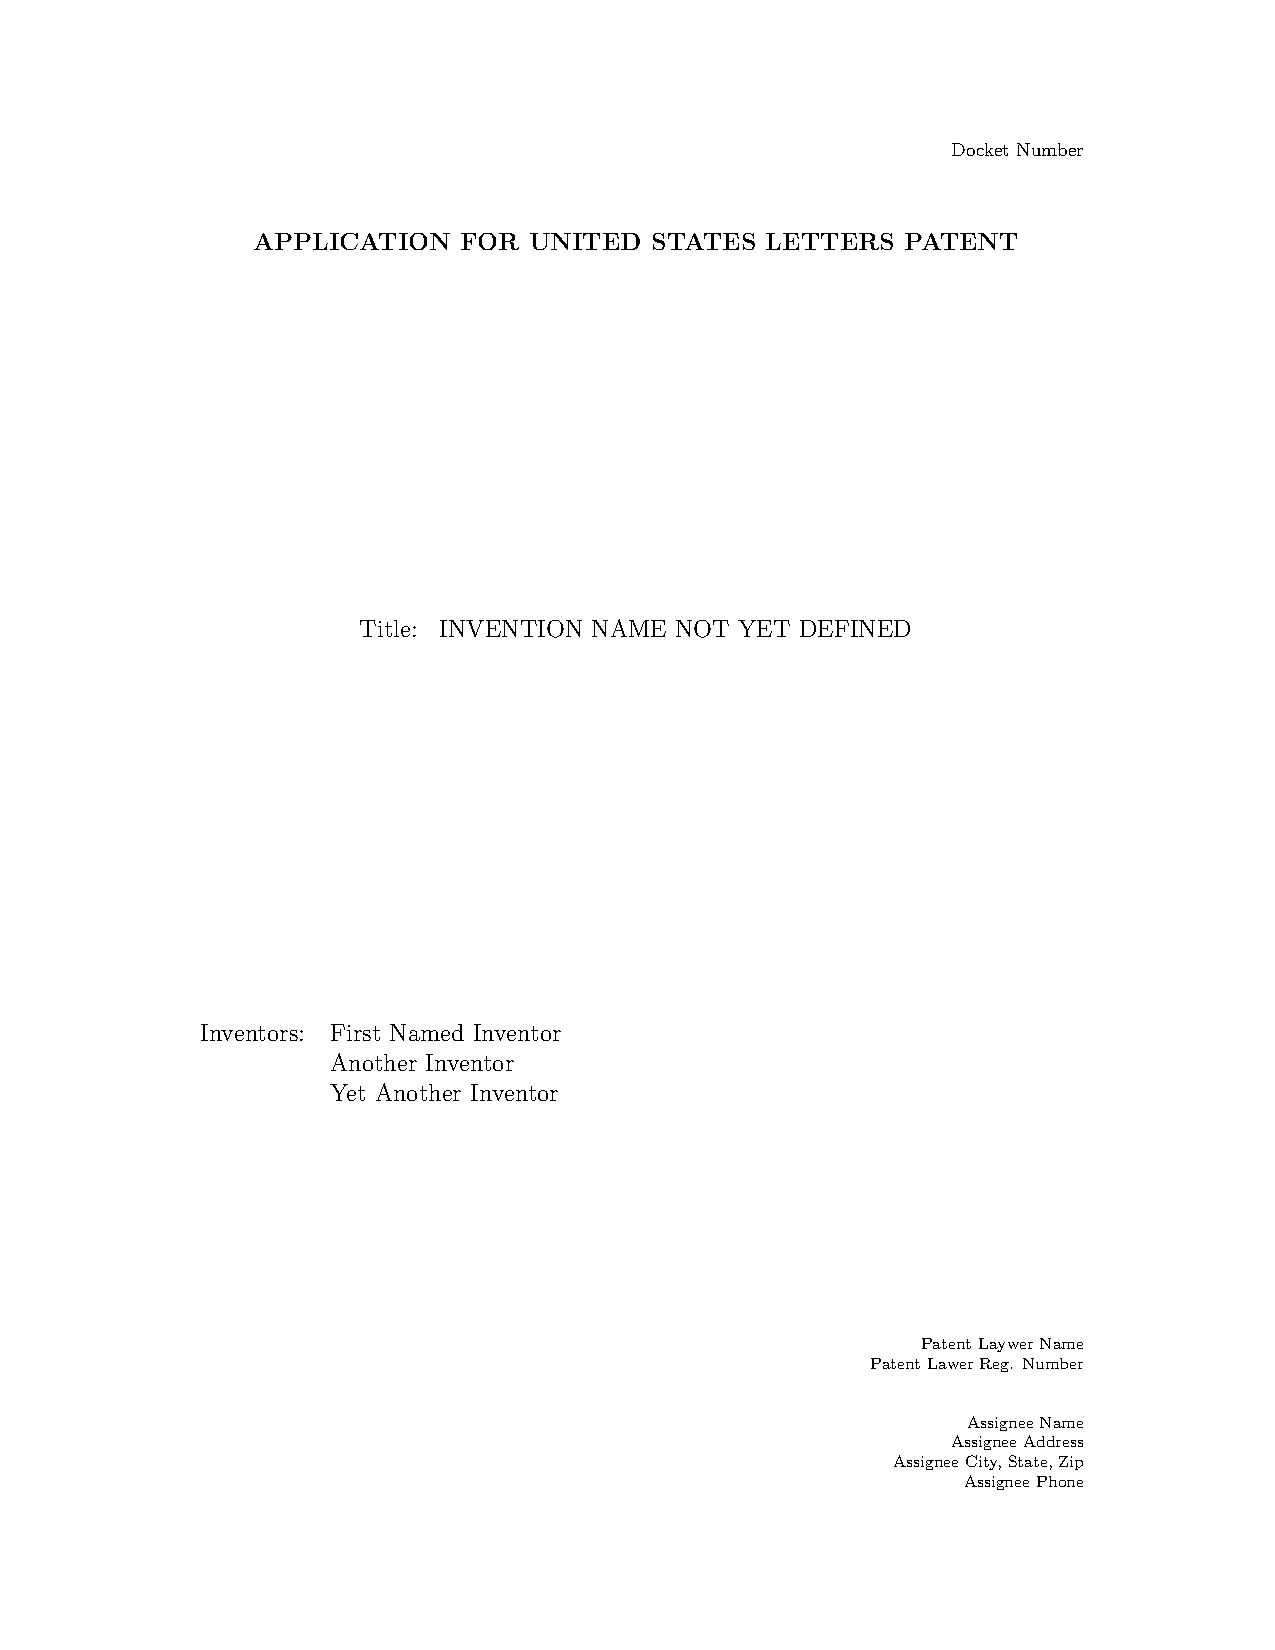
\includepdf[pages=-]{PatentApplication}

\cleartooddpage

\noindent \printindex{}
\end{document}
